%%%%%%%%%%%%%%%%%%%%%%%%%%%%%%%%%%%%%%%%%%%%%%%%%%%%%%%%%%%%%%%%%%%%
\section{Introduction}
%%%%%%%%%%%%%%%%%%%%%%%%%%%%%%%%%%%%%%%%%%%%%%%%%%%%%%%%%%%%%%%%%%%%
\label{sc:Intro}

Only six terrestrial bodies in our solar system (Venus, Earth, Mars, Titan, Triton, Pluto)
 possess an atmosphere thick enough to be governed
by the same equations of meteorology as on Earth, or able to support clouds or hazes. 
Among them, Pluto presents a unique case, with an atmosphere significantly warmer than the
underlying surface, long radiative timescales, and a circulation dominated by
condensation/sublimation process of the main atmospheric component. Studying this exotic 
case can provide new insight into the physics of terrestrial atmosphere. 

The observations made by the New Horizons spacecraft have 
revealed the nature of the surface of Pluto
and have provided unprecedented constraints on the state of the atmosphere in 2015
\citep{Ster:15,Glad:16,Grun:16,Moor:16}.
Within that context, it is now interesting to test our ability to create a 
3D numerical simulator of the Pluto climate system, analogous to the climate models already 
used on the Earth as well as on Mars, Venus and Titan.  
Conversely, the output of  such a Global Climate Model is useful to interpret the
available atmospheric measurements, and can even shed light on some geological observations.


\subsection{Pluto's ices and atmosphere observations}

The presence of a significant atmosphere on Pluto was demonstrated in 1988 by observing 
a stellar occultation by Pluto
\citep{Hubb:88,Elli:89}. This atmosphere was predicted 
to be mainly composed of molecular nitrogen in 
vapour-pressure equilibrium with N$_2$ ice deposits observed on the surface. 
In 2015, New Horizons determined a pressure of about 10~$\mu$bar, i.e. 1~Pa \citep{Hins:15dps,Glad:16}. 
However,  a series of stellar occultations conducted since 1988 have shown
that the pressure at a specific reference level (e.g. 1275~km 
from Pluto's center) has increased by a factor of three during that
period \citep{Elli:03,Sica:03,Olki:15}, suggesting a
similar rise of the surface pressure. 

Prior to the New Horizons flyby, spectroscopic observations 
had demonstrated that, in addition to N$_2$ ice, Pluto's surface is covered by patches of
CH$_4$ and CO ices \citep{Owen:93,Dout:99,Grun:13}. 
New Horizons was able to map these ices and revealed that the main reservoir was a
thick ice cap informally named Sputnik Planum, with thinner 
N$_2$ frost covering the
mid-northen latitudes and CH$_4$ frost possibly everywhere except in the equatorial dark regions
\citep{Grun:16}. 

Accordingly, CH$_4$ and CO gas were observed from Earth to be present in present-day 
Pluto's atmosphere 
\citep{Youn:97,Lell:09,Lell:11co,Lell:15,Lell:16},
with, during the 2008-2012 period,
volume mixing ratios near 
0.05\% for CO and 0.5\% for CH$_4$.
\citep{Lell:11co,Lell:15}.
CH$_4$ has also been oberved by New Horizons Alice spectrograph.
in 2015 and estimated to range between 0.6 and 0.84~\% in the lower
atmosphere \citep{Glad:16}.
Using the hydrostatic equation, atmospheric temperature profiles 
have been derived from vertical density profiles 
retrieved from Earth-based stellar occultations
\citep{Elli:89,Sica:03,Elli:07,Pers:08,Youn:08,Dias:15,Sica:16}, and  from 
radio and solar occultations performed by New Horizons \citep{Hins:15dps,Glad:16}.
The latest stellar occultations and New Horizon's data consistently show that 
the temperature profile is characterized by a steep temperature gradient 
in the lower atmosphere, 
with temperature increasing from surface values (38 to 55~K) at 0~km 
to about 110~K at 20~km. 
This has been interpreted as resulting from the absorption of near-infrared solar radiation
by gaseous methane \citep{Yell:89,Stro:96}. 
Above 30~km, the temperature appears to decrease with altitude 
to reach about 70-80~K around 200~km \citep{Dias:15,Gurw:15dps,Glad:16}. 
Such a structure requires
infrared-cooling species acting only at a specific altitude range. 
C$_2$H$_2$ and HCN --~respectively
detected by New Horizons \citep{Glad:16} and from the ground
\citep{Lell:16}~--
have been proposed, but the details of exactly how Pluto’s upper atmosphere is
being cooled remains poorly understood \citep{Glad:16}. 
Finally, stellar occultation observations suggest
that the temperature profiles are affected by oscillation that can be related to gravity waves or
thermal tides \citep{Sica:03,Pers:08,Toig:10}.

\subsection{3D Modelling of the Pluto surface-atmosphere system}

To improve our understanding of the complex Pluto surface-atmosphere system,
we have built a new Global Climate Model (GCM) including a full simulation
of the nitrogen, methane, and carbon monoxide cycles. 
This GCM computes the temporal evolution of the variables which control 
the meteorology and the climate of the planet in different points of a 3D grid
covering the entire atmosphere. On the Earth, GCMs have been applied to weather
forecasting and climate change projections.
Because these models are almost entirely built on
physical equations (rather than empirical parameters),
several teams around the world have been able to succesfully adapt them
to the other terrestrial planets or satellites that have a
solid surface and a thick enough atmosphere. The Pluto GCM presented
in this paper is derived from the LMD Global Climate Model of planet Mars (Forget
et al. 1999) which has been used for numerous applications including simulating CO$_2$
ice caps analogous to Pluto's N$_2$ ice caps (Forget et al. 1998),
the thermosphere (Gonzalez-Galindo et al., 2009), photochemistry
(Lefevre et al. 2008) or paleoclimatology (e.g. Forget et al. 2006).
The LMD GCM has been
adapted to Venus (Lebonnois et al., 2010)
and Titan (Hourdin et al. 1995, Lebonnois et al. 2012).
All these GCMs have been able to predict or accurately reproduce the
observed thermal structure and circulation, giving us some confidence in its
ability to predict the characteristics of the Pluto atmosphere in spite of the scarcity of
observations.
\nocite{Lebo:10,Hour:95,Lebo:12,Forg:06,Forg:99,Forg:98,Gonz:09a}

For Pluto, after the simplified General Circulation Model (without phase changes) 
presented by \cite{Zalu:13} for Pluto and Triton, a realistic model was developed
by \cite{Toig:15} a few months before the New Horizons encounter. This model includes a
``robust treatment of nitrogen volatile transport'', and initializes
the full GCM using a two dimensional surface volatile exchange model and a 
one-dimensional radiative-conductive-convective model. 
In this paper we present a new model with a different origin and which benefits 
from the New Horizons observations. We include 
an improved N$_2$ condensation-sublimation scheme, the full CO and CH$_4$ cycles, and 
explore the effect of topography.  Nevertheless, we use an analogous strategy
for the initialization. 

In Sections~\ref{sc:model}, we  provide a detailed description of the different components of
our Pluto Global Climate Model, and in Section~\ref{sc:initial} we discuss how the
different model parameters were chosen and how the 3D GCM is initialized for our two
baseline simulations. The model results for temperature and winds and for the CH$_4$ and
CO cycles are then presented in Sections~\ref{sc:Tresults} and~\ref{sc:ch4_co_results},
before the conclusion. 


%%%%%%%%%%%%%%%%%%%%%%%%%%%%%%%%%%%%%%%%%%%%%%%%%%%%%%%%%%%%%%%%%%%%
\section{Model description}
%%%%%%%%%%%%%%%%%%%%%%%%%%%%%%%%%%%%%%%%%%%%%%%%%%%%%%%%%%%%%%%%%%%%
\label{sc:model}
\label{sc:physi}

%%%%%%%%%%%%%%%%%%%%%%%%%%%%%%%%%%%%%%%%%%%%%%%%%%%%%%%%%%%%%%%%%%%%
\subsection{Generalities}
%%%%%%%%%%%%%%%%%%%%%%%%%%%%%%%%%%%%%%%%%%%%%%%%%%%%%%%%%%%%%%%%%%%%

\label{sc:dynam}
\label{sc:dynamic}

As mentioned above, our Pluto Global Climate Model is derived from the LMD Mars GCM 
\cite[]{Forg:99} , with several new parameterizations.
Its core is a hydrodynamical code dedicated to the temporal and spatial integration of the
equations of hydrodynamics, used to compute the large scale atmospheric motions and the
transport.  The equations are solved using a finite difference scheme on an ``Arakawa C'' grid
\cite[]{Arak:77}.
Such a scheme is equally valid for the Earth, Mars or Pluto. Therefore the hydrodynamical
core
 has not been
modified for Pluto.  While the estimated surface pressure on Pluto (10~$\mu$bar or 1~Pa)
is much lower than on the Earth or even on Mars, the atmosphere is thick
enough to be modeled with the primitive equations of meteorology used in the
model. In fact, it is generally found that GCMs dynamical cores are valid almost up to the
exobase.
For instance, on Mars our dynamical core has been used sucessfully up to
the thermosphere at pressures lower than 10$^{-7}$~Pa
\cite[]{Gonz:09a}.

In this paper, we present simulations with a horizontal grid of 
32$\times$24
points to cover the planet,
that is a grid-point spacing 
of 7.5$^{\circ}$ latitude by 11.25$^{\circ}$ longitude.
The corresponding
spatial resolution is of about 150~km, which is equal or better to the typical resolution used in
planetary GCMs, and which is sufficient to resolve possible planetary waves. We also performed
simulations with a doubled resolution (64$\times$48) and even an experimental  run 
with a 360$\times$180 
grid, and did
not find any fundamental differences in the results that could change the conclusions of this
paper. Their analysis is out of the scope of this paper and will be presented in a future article,
in which we will take into account a more realistic topography.  
In the vertical, the model uses the terrain-following ``sigma''
coordinate system in finite difference form (i.e. each layer is defined by a constant value
of the ratio pressure devided by surface pressure). 25 levels are typically used.
In the baseline model,
most of the levels are located in the first 15 km to obtain a good resolution close 
to the surface, in the boundary layer. The altitude of the first mid-layers are 7~m, 15~m, 25~m,
40~m, 80~m etc.. Above 10~km, the resolution is about one scale height, with the upper pressure 
level equal to 0.007 times surface pressure, i.e. up to 250~km. (Note that in a companion paper dedicated to the study of 
atmospheric hazes \cite{Bert:16ica}, the top of the model is 
extended to about 600~km to include the altitudes of methane photolysis). 


%%%%%%%%%%%%%%%%%%%%%%%%%%%%%%%%%%%%%%%%%%%%%%%%%%%%%%%%%%%%%%%%%%%%
\subsection{Radiative transfer}
%%%%%%%%%%%%%%%%%%%%%%%%%%%%%%%%%%%%%%%%%%%%%%%%%%%%%%%%%%%%%%%%%%%%

\label{sc:radia}

The incident insolation upon each modeled atmospheric 
column is calculated at each timestep, taking into
account the variation of the Pluto-Sun distance throughout its orbit, the seasonal
inclination and the diurnal cycle. 

While N$_2$ is the major constituent of the atmosphere of Pluto, its
radiative effects are neglected in the lower atmosphere since
N$_2$ is transparent at solar and infrared wavelengths. 
Nevertheless we account for (1) the radiative
heating and cooling by CH$_4$, which can vary in space and time depending of the results of the
methane cycle model (see section~\ref{sc:ch4_model}) (2) cooling by the thermal infrared 
rotational lines of CO, which volume mixing ratio is prescribed at 0.05~\%
everywhere \cite[]{Lell:11co,Lell:16} and 3) the effect of other infrared emitting species in altitude.  

\subsubsection{Radiative transfer through CH$_4$ and CO}
For CH$_4$ and CO, we use a correlated $k$-distribution radiative transfer model, 
with 17 spectral bands in the thermal infrared and 23 for solar wavelengths. The bands are
designed to well represent the 1.6, 2.3 and 3.3~$\mu$m CH$_4$ vibrational bands in the near
infrared as well as the 7.6~$\mu$m CH$_4$ emission band in the thermal infrared.
To calculate the $k$ absorption coefficients in each bands, 
high resolution line-by-line spectra combining CO and CH$_4$  
were computed from the HITRAN 2012 database using the open-source ``kspectrum'' tool.
Spectra and $k$ coefficients were calculated to fill
a look up table matrix (from which the $k$ coefficients are interpolated by the GCM in each
spectral band) comprising  8~temperatures $\times$ 7~log-pressure $\times$
7~CH$_4$ volume mixing ratio grid, with 
$T=\{30, 40, 50, 70, 90, 110, 150, 200\}$~K, 
$p=\{10^{-4}, 10^{-3}, 10^{-2}, 10^{-1}, 1, 10, 100\}$~Pa, and
[CH$_4$]= $\{10^{-4},  10^{-3}, 5\times10^{-3},
10^{-2}, 5\times10^{-2},
10^{-1}, 5\times10^{-1}\}$~kg/kg. 
We found that no less than 33 points were needed for the $g$-space integration to get accurate
results throughout the matrix space ($g$ is the cumulated distribution
function of the absorption data for each band).  

\subsubsection{Non Local Thermal Equilibrium processes}
In the low-pressure, low temperature Pluto environment, a major difficulty (and therefore
uncertainty) in the radiative transfer calculations results from the fact that the methane
lines can be far from Local Thermal Equilibrium (LTE). It is not the case of 
CO rotational lines which are assumed to
remain in LTE for the pressure levels that we model in this paper. 

To account for non-LTE effects for the 7.6~$\mu$m CH$_4$ band, we modify the LTE
cooling rates obtained with the correlated $k$-distribution radiative transfer model as in
\cite{Stro:96}. However, the total CH$_4$ cooling rates we obtain are found to be 
much lower than shown in \cite{Stro:96}, and significantly smaller than the CO cooling rates. 
This is also found in recent models from the same authors (D. Strobel, personnal communication)
The difference is thought to result from the updated spectroscopic database (HITRAN 2012 vs
HITRAN 1986) and the fact that the temperatures used in \cite{Stro:96}  are larger than here.
The uncertainties on the NLTE calculations for the 7.6~$\mu$m CH$_4$ band have thus 
a limited effect on our results.

For the near-infrared solar bands, we first reproduced the calculations from
\cite{Stro:96} updated by \cite{Zalu:11} for each of the 2.3 and 3.3~$\mu$m bands. 
We had no information on the 1.6~$\mu$m band.  Within that context, 
and given the overall uncertainty in the NLTE calculations \citep{Bour:03}, 
we authorized some empirical
modifications of the theoretical NLTE variations with atmospheric density (while
keeping the theoretical shape) to adjust the heating rates in order to get
temperatures closer to the thermal structure observed by New Horizons. Therefore, the ability of
our GCM to roughly reproduce the observed mean thermal structure should not be regarded as a
success of our radiative transfer model. 
In practice, we multiply the total CH$_4$ heating rate provided by the LTE radiative
transfer code by a vertically varying non-LTE efficiency coefficient 
$\varepsilon_{\mbox{\scriptsize NLTE}}$. 

\begin{equation}
\varepsilon_{\mbox{\scriptsize NLTE}} = 0.1 + \frac{0.9}{1+{\rho_{\mbox{\scriptsize .55}}}/{\rho}}, 
\end{equation}
with $\rho$ the atmospheric density (kg\ m$^{-3}$), and $\rho_{\mbox{\scriptsize .55}}$ the reference
density for which $\varepsilon_{\mbox{\scriptsize NLTE}}=0.55$. 
After tuning, we set $\rho_{\mbox{\scriptsize .55}}=2\times10^{-6}$~kg~ m$^{-3}$.

\subsubsection{Additional radiative coolers}

As mentioned in the introduction, the presence of radiatively cooling species at a 
specific altitude
has been suggested to explain the decrease of temperature above 30~km 
\citep{Dias:15,Glad:16}. Using the cooling-to-space approximation, we phenomenologically
represent this
effect with the following cooling rate for pressures below 0.12~Pa:

\begin{equation}
\frac{\partial T}{\partial t} = -5\times10^{-11} \   B(\lambda_0,T) 
\end{equation}

with $T$ the atmospheric temperature (K) and $B(\lambda_0,T)$ the Planck function (in
W~m$^{-2}$~$\mu$m$^{-1}$~sr$^{-1}$) at wavelength $\lambda_0$. We use $\lambda_0 =
14$~$\mu$m since the main emission bands of the most likely cooling species 
 C$_2$H$_2$ and HCN \citep{Glad:16} are respectively centered at 13.7 and 14.05~$\mu$m
(we here neglect the rotational bands of HCN at submillimeter wavelengths).
The value $-5\times10^{-11}$ was chosen to simulate a moderate cooling yielding temperatures below 90~K
in our reference simulation.


%%%%%%%%%%%%%%%%%%%%%%%%%%%%%%%%%%%%%%%%%%%%%%%%%%%%%%%%%%%%%%%%%%%%
\subsection{Atmospheric molecular thermal conduction and viscosity}
%%%%%%%%%%%%%%%%%%%%%%%%%%%%%%%%%%%%%%%%%%%%%%%%%%%%%%%%%%%%%%%%%%%%
\label{sc:acond}

We account for the effect of molecular conduction on temperature and molecular 
viscosity on winds.  Both processes are governed by similar equations.
Assuming the plane-parallel approximation, for  thermal conduction we get:

\begin{equation} 
\frac{\partial T}{\partial t}=\frac{1}{\rho 
c_p}\frac{\partial}{\partial z}\left(k\frac{\partial T}{\partial z}\right) 
\end{equation}

where $T$ is the temperature (K), $\rho$ the density (kg~m$^{-3}$) and $k$ the
thermal conduction coefficient (J m$^{-1}$ s$^{-1}$ K$^{-1}$), expressed as
$k = k_0 T^{s}$, with 
$k_0 = 5.63\times10^{-5}$~J~m$^{-1}$~s$^{-1}$~K$^{-(1+s)}$ 
and $s=1.12$ \citep{Hubb:90}. 

For molecular viscosity:

\begin{equation} \frac{\partial S}{\partial 
t}=\frac{1}{\rho}\frac{\partial}{\partial z}\left(\mu \frac{\partial S}{\partial 
z}\right) 
\end{equation}

where $S$ stands for the components of the horizontal wind
(m~s$^{-1}$) 
and $\mu$ is the coefficient of molecular viscosity (kg m$^{-1}$ s$^{-1}$), that
is related to the thermal conduction coefficient by $k=\frac{1}{4}[9c_p-5(c_p-R)]\mu$.
Given its similarity, both equations are discretized
and solved using the same implicit numerical schemes.


%%%%%%%%%%%%%%%%%%%%%%%%%%%%%%%%%%%%%%%%%%%%%%%%%%%%%%%%%%%%%%%%%%%%
\subsection{Surface temperatures and thermal conduction in the subsurface}
%%%%%%%%%%%%%%%%%%%%%%%%%%%%%%%%%%%%%%%%%%%%%%%%%%%%%%%%%%%%%%%%%%%%
\label{sc:csoil}

Surface temperature evolution $T_s$ is governed by the balance between solar
insolation, thermal emisssion in the infrared, 
%($\epsilon\sigma T_s^4$ W m$^{-2}$ with $\sigma=5.67\times10^{-8}$ 
% and $\epsilon$ the surface emissivity)
latent heat exchanges (see section~\ref{sc:cond}), sensible heat flux from the
atmosphere (usually negligible on Pluto, but taken into account in the model) 
and thermal conduction in the soil.
On a weakly irradiated body like Pluto, the radiative fluxes are small compared to the
internal heat stored in the ground. In particular, the subsurface heat stored during one
season can play a major role in the control of the surface temperature
at the opposite season.

The heat flux from and to the subsurface is computed using a classical
model of the evolution of the subsurface temperatures $T$
as a function of time $t$ and depth $z$.  It satisfies the following equation:
\begin{equation} \label{eq:Heat1D}
C \frac{\partial T}{\partial t} =
\frac{\partial }{\partial z}
\left[ \lambda \frac{\partial T}{\partial z} \right]
\end{equation}

where $\lambda$ is the heat conductivity of the ground,
(J s$^{-1}$ m$^{-1}$ K$^{-1}$) and
$C$ the ground volumetric specific heat (J m$^{-3}$ K$^{-1}$).
This equation is solved using a finite differences approach and an implicit Euler
scheme.  
The key parameter which  controls the influence of the subsurface heat
storage and conduction on the surface temperature is the thermal Inertia
$I = \sqrt{\lambda C} $. In practice, we thus use $I$ as the key model
parameter, assuming a constant value for C=10$^6$ J m$^{-3}$ K$^{-1}$ and making
$\lambda$ vary accordingly.


On Pluto the discretization requires a special attention compared to the Earth or Mars
because one need to simultaneously capture 1) the short period 
diurnal thermal waves in the near-surface, low thermal inertia terrain and 2) the
much longer seasonal thermal waves which can penetrate deep in the high thermal inertia
substrate.  
In this paper, we assumed a relatively 
low diurnal thermal inertia $I_{\mbox{\scriptsize day}}=50$~J s$^{-1/2}$ m$^{-2}$
K$^{-1}$, slightly higher than the 20 to 30 SI range reported by 
\cite{Lell:11spitzer} from their Spitzer data analysis. For the 
seasonal thermal inertia, we set  $I_{\mbox{\scriptsize year}}=800$~J s$^{-1/2}$ m$^{-2}$
K$^{-1}$, which corresponds to a low porosity ice/rock-like substrate. 

The skin depth of a thermal wave of period $P$ (s) is:
\begin{equation}
\delta_{P} =  \frac{I}{C} \sqrt{\frac{P}{\pi}}
\end{equation}

The modeled diurnal and annual skin depths are thus 0.02~m and 40~m respectively.
To represent this accurately, the subsurface is divided into $N=22$ discrete 
layers, with a geometricaly stretched distribution of layers 
with higher resolution near the surface and
a  coarser grid at depth:
\begin{equation}
z_k = z_1 \, 2^{k-1}
\end{equation}
where $z_1 = 1.414 \times 10^{-4}$~m is the depth of the first layer. 
The deepest layer depth is thus near 300~m.

%%%%%%%%%%%%%%%%%%%%%%%%%%%%%%%%%%%%%%%%%%%%%%%%%%%%%%%%%%%%%%%%%%%%
\subsection{Mixing in the boundary layer}
%%%%%%%%%%%%%%%%%%%%%%%%%%%%%%%%%%%%%%%%%%%%%%%%%%%%%%%%%%%%%%%%%%%%
\label{sc:subgr}
\label{sc:pbl}


Turbulent mixing and convection are parameterized
as in \cite{Forg:99}.  In practice, the boundary layer
dynamics is accounted for by a \cite{Mell:82}
unstationary 2.5-level closure scheme, used to compute turbulent mixing
coefficients induced by wind shears depending
on the temperature profile stability and the evolution of turbulent kinetic energy. 
It is completed by a ``convective adjustment'' scheme  which rapidly mixes the
atmosphere in the case of unstable temperature profiles (rare on Pluto).

Turbulence and convection mix
energy (potential temperature), momentum (wind), and tracers (gases and aerosols).
In the surface layer, the turbulent surface flux is given by
\begin{equation}
F = \rho C_d  U_1 (q_1 -q_0), 
\label{eq:sflux}
\end{equation}
where $q_1$ and $q_0$ are the variable values
in the first atmospheric layer and at the surface ($q_0=0$ for winds),
$U_1$ is the horizontal wind velocity in the first layer, and $ C_d$ is the drag
coefficient. Because of the small depth of the first layer
$z_1$, we assume that the wind profile in the first meters
above the surface is logarithmic and not influenced by stability, and simply  use
\begin{equation}
C_d = \left( \frac{\kappa}{\ln{\frac{z_1}{z_0}}} \right)^2
\end{equation}
where $\kappa$ is the von Karman
constant ($\kappa$ = $0.4$) and  $z_{0}$ is the
roughness coefficient, set to $z_{0}=0.01$~m everywhere like in the Mars GCM
\citep{Forg:99}.

%Tests results show a negligible influence of $z_{0}$ on the model.

Turbulent mixing is negligible outside the boundary layer (which is often shallow on Pluto because of the positive lapse
rate above the surface). In our GCM there is no other vertical ``eddy diffusion'' 
process. In particular, species are only 
transported upwards by the large scale circulation.



%%%%%%%%%%%%%%%%%%%%%%%%%%%%%%%%%%%%%%%%%%%%%%%%%%%%%%%%%%%%%%%%%%%%
\subsection{N$_2$ Condensation and Sublimation}
%%%%%%%%%%%%%%%%%%%%%%%%%%%%%%%%%%%%%%%%%%%%%%%%%%%%%%%%%%%%%%%%%%%%
\label{sc:cond}
\def\dem{\frac{1}{2}}

The condensation and sublimation of nitrogen ice must be carefully computed in the
Pluto environment. The amount of energy and the relative mass of the atmosphere
involved in phases changes at each timestep can be very significant. 
Locally, it not only changes
the surface temperature and pressure, but it also modifies the structure of the
boundary layer by "pumping" the air when condensation occurs on the surface,
and by releasing large amount of cold, pure nitrogen (with no horizontal velocity)
when N$_2$ sublimes. 
Our scheme is adapted from \citet{Forg:98}. However, we found it necessary to 
make several changes in the equations to better represent the 
intense condensation and sublimation at the surface of Pluto.

The variation of the condensation temperature $T_c$ with nitrogen partial
 pressure $P_{\mbox{\scriptsize N2}}$  is derived from the thermodynamic relations computed by 
 \cite{Fray:09},
taking into account the transition from the $\alpha$ to the $\beta$ crystalline form near 35.61~K
(corresponding to $P_{\mbox{\scriptsize N2}}=0.53$~Pa):

%     FORTRAN ORIGINAL CODE:
%     IF (p.ge.0.529995) then
%  !   tcond Fray and Schmitt for N2 phase beta (T>35.6 K) FIT TB15
%      tcond_n2 = ( (1./63.1470) -(296.925/(2.5e5*0.98))*log(p/(0.125570*1.e5))   )**(-1)
%     ELSE
%  !   tcond Fray and Schmitt for N2 phase alpha(T<35.6 K) FIT TB15
%      tcond_n2 = ( (1./35.6) -(296.925/(2.5e5*1.09))*log(p/0.508059)   )**(-1)
%     ENDIF

\begin{eqnarray}
\mbox{if } P_{N2} <0.53 \mbox{ Pa :} & 
T_c  = &  \left[ \frac{1}{35.600} - \frac{296.925}{1.09 L_{\mbox{\scriptsize N2}}} 
\ln{\left( \frac{P_{\mbox{\scriptsize N2}}}{0.508059} \right) } \right]^{-1} 
\\
\mbox{if } P_{N2} >0.53 \mbox{ Pa :} & 
T_c  = & \left[ \frac{1}{63.147} - \frac{296.925}{0.98 L_{\mbox{\scriptsize N2}}} 
\ln{ \left( \frac{P_{\mbox{\scriptsize N2}}}{12557.}\right) } \right] ^{-1} 
\end{eqnarray}

with $L_{\mbox{\scriptsize N2}} =2.5.10^{5}$~J~kg$^{-1}$ the latent heat of
condensation for nitrogen.
 
\subsubsection{Surface Condensation and sublimation}

The condensation and sublimation of nitrogen on the ground
is primarily controlled by energy and mass conservation.
At a given timestep,  if the surface temperature predicted by radiative and
conductive balance $T_0^*$ falls below the 
condensation temperature at surface pressure $T_c0$, 
an amount 
$\delta m_0$ (kg~m$^{-2}$) of N$_2$ condenses, releasing
the latent heat required to keep the solid-gas interface at the condensation
temperature ($T_0 = T_{c0}$):

\begin{equation}
\label{eq:condatm}
\delta m_0 = \frac{c_s}{(L_{\mbox{\scriptsize N2}}  +c_p(T_1 -T_{c0}))} (T_{c0} - T^*_0) 
\end{equation}

$c_s$ is the surface heat capacity (in J~m$^{-2}$~K$^{-1}$), 
$c_p$  the air specific heat at constant pressure
(set to 1040~J~kg$^{-1}$~K$^{-1}$ for N$_2$) and $L_{\mbox{\scriptsize N2}} $ the latent
heat of N$_2$ ($2.5~10^5$~J~kg$^{-1}$). 

The term $c_p(T_1 -T_{c0})$ (J~kg$^{-1}$) corresponds to the extra heat brought by the
atmosphere (assumed to be at temperature $T_1$ in the first model layer) when cooled
to the condensation temperature $T_{c0}$ just above the surface.
Because Pluto's lower atmosphere is a warm stratosphere lying just above a
surface, 
we found that this term can be significant. With $T_1$ typically 10~K above 
$T_{c0}$ when N$_2$ condenses in the topics, it reaches 4\% of the latent heat. 
Conversely, when surface N$_2$ ice predicted temperature 
$T^*_0$ is above the frost point $T_{c0}$, N$_2$ sublimes
and $\delta m_0$ is negative:

\begin{equation}
\delta m_0 = \frac{c_s}{L_{\mbox{\scriptsize N2}} } (T_{ca}0 - T^*_0) 
\end{equation}

We set $T_0 = T_{c0}$, unless all the local ground ice of mass $m_0$ (kg~m$^{-2}$)
completely sublimes. We then set $\delta m_0 = -m_0$ and
the new surface temperature is expressed as:
$T_0 = T^*_0 - L_{\mbox{\scriptsize N2}}  \ m_0 / c_s $
The formation or disapearance of nitrogen ice on the substrate is taken into
account in the calculations of the surface albedo and emissivity.

\subsubsection{Atmospheric Condensation and sublimation}

In the atmosphere, things are, in theory, more complex.
The condensation of a gas involves various
microphysical processes: supersaturation,  nucleation,
crystal growth, sedimentation, etc...
In our model, we have kept the detailed Mars GCM CO$_2$ ice sheme described in
the appendix of \citet{Forg:98} and directly adapted it to N$_2$ ice.
Supersaturation is neglected and
atmospheric condensation and sublimation are computed using energy
conservation principles as above. 
We do not simulate the growth and transport of nitrogen ice particles.
Instead, after condensing at a given model level, we assume that
N$_2$ ice falls through the atmospheric layers
located below it (where it can sublimate),
possibly down to the ground within a model timestep.

Because the atmosphere is warmer than the surface most of the time, we have found
that atmospheric condensation is a processes of little importance on Pluto as we
model it with a 150~km resolution. In reality, ascending motions induced by local
slopes or gravity waves could trigger condensation in N$_2$ ice covered regions. 
We will explore that in future versions of the model. 

\subsubsection{Computing mass, momentum and heat vertical fluxes induced by N$_2$
condensation and sublimation}

The condensation and sublimation of nitrogen
induce significant transport of air (mass, heat, momentum, tracers)
through the model layers as well as to and from the surface. 
These processes must be taken into account on Pluto 
where an atmospheric layer of several tens of  meters thick can undergo a phase change 
at each timestep. The numerical resolution of these processes in the 
``$\sigma$'' vertical coordinates used in the GCM (see Section~\ref{sc:dynamic}) 
is given in the appendix. 

%%%%%%%%%%%%%%%%%%%%%%%%%%%%%%%%%%%%%%%%%%%%%%%%%%%%%%%%%%%%%%%%%%%%
\subsection{Organic hazes}
%%%%%%%%%%%%%%%%%%%%%%%%%%%%%%%%%%%%%%%%%%%%%%%%%%%%%%%%%%%%%%%%%%%%

New Horizons revealed the presence of extensive hazes thought to be primarily
composed of organic particles indirectly produced by methane photolysis. Our GCM
includes a model of the formation and transport of these particles. This model and
its outputs are described and analyzed in a companion paper by \cite{Bert:16ica}, and
not detailed here.


%%%%%%%%%%%%%%%%%%%%%%%%%%%%%%%%%%%%%%%%%%%%%%%%%%%%%%%%%%%%%%%%%%%%
\subsection{Methane cycle and CH$_4$ ice clouds}
%%%%%%%%%%%%%%%%%%%%%%%%%%%%%%%%%%%%%%%%%%%%%%%%%%%%%%%%%%%%%%%%%%%%
\label{sc:ch4_model}

The 3D evolution of CH$_4$ on the surface and in gaseous and solid phase in 
the atmosphere is simulated taking into account 1) the condensation and sublimation at the
surface and in the atmosphere (see below),
2) the transport by the general circulation using the ``Van-Leer~I'' finite volume scheme from \cite{Hour:99}, 
3) the mixing in the atmosphere by turbulent diffusion and possibly convection (see
Section~\ref{sc:pbl}), and 
4) the gravitational sedimentation of CH$_4$ ice particles (see below).  

\subsubsection{Surface condensation and sublimation.}

The mass fluxes of methane to and from the atmosphere are computed using 
Eq.~\ref{eq:sflux}, with $q_0$ and $q_1$ the mass mixing ratios  (kg/kg)
just above the surface and in the middle of the atmospheric first layer, respectively.
Note that an important consequence of Equation~\ref{eq:sflux} 
is that the sublimation rate of methane is 
proportional to the horizontal wind velocity in the lower atmosphere. 

When pure methane is on the surface, $q_0$ is set equal to the saturation vapour pressure 
mass mixing ratio of methane $q_{\mbox{\scriptsize  sat CH4}}$, 
calculated as a function ot temperature $T$ (K) and pressure $p$
using the following expression derived from \cite{Fray:09}:
%     ORIGINAL FORTRAN MMR
%    qsat(i)=0.117.E5*exp((16*612.5/8.314)*(1/90.7-1/t(i)))

\begin{equation}
q_{\mbox{\scriptsize sat CH4}} = 0.117 \times 10^{5}  
%e^{{\frac{612.5}{R}} 
e^{{\frac{6.12 \times 10^{5}}{R}} 
\left(  {1}/{90.7} -{1}/{T} \right) } 
\times \frac{M_{\mbox{\scriptsize CH4}}}{M_{\mbox{\scriptsize air}}} \times \frac{1}{p}
\label{eq:ch4sat}
\end{equation}

Here ${M_{\mbox{\scriptsize CH4}}}/{M_{\mbox{\scriptsize air}}}$ is the ratio of molecular masses use
to convert volume mixing ratio into mass mixing ratio and  
$R = 8.314/M_{\mbox{\scriptsize CH4}} = 519~$~m$^2$~s$^{-2}$~K$^{-1}$ the methane gas constant.
When both methane and nitrogen ices are 
present on the surface and methane is subliming, we assume that methane is diluted in a solid solution N$_2$:CH$_4$
with 0.3\% of methane \citep{Merl:15}. Applying Raoult's law, we thus set $q_0= 0.005
q_{\mbox{\scriptsize  sat CH4}}$
If the total amount of methane on the surface is sublimed within a model timestep, the flux to the atmosphere is limited accordingly. 
If no methane ice is present on the surface, then $q_0= q_1$ if $q_1 <
q_{\mbox{\scriptsize sat CH4}}$ (no condensation) and 
$q_0 = q_{\mbox{\scriptsize sat CH4}}$ if $q_1 > q_{\mbox{\scriptsize sat CH4}}$ (direct condensation onto the surface).
The latent heat released by methane surface condensation and sublimation is taken into account 
in the surface energy budget
assuming a latent heat $L_{\mbox{\scriptsize CH4}} = 5.867 \times 10^5$~J~kg$^{-1}$
 \cite[]{Fray:09}.


\subsubsection{Atmospheric condensation and CH$_4$ cloud formation}

Methane can also condense (and then sublimate) 
in the atmosphere when the CH$_4$ mixing ratio exceeds the saturation mixing ratio provided by 
Equation~\ref{eq:ch4sat}. We do not know if CH$_4$ 
can easily nucleate or if large super-saturation 
is required. Organic
particles resulting from the photochemistry in the upper atmosphere probably offer condensation nuclei suitable for heterogeneous condensation.
In the GCM we assume that all atmospheric methane in excess of saturation 
condenses to form ice cloud particles.

The amount of latent heat released by methane condensation or sublimation is 
far from being negligible. We find that it can locally change the
atmospheric temperature by more than 10~K. Moreover, latent heating  actually limits
the amount of methane that condenses when the atmosphere is supersaturated. 
If CH$_4$ condensation is calculated
without simultaneously taking into account latent heat release, 
or using an explicit numerical scheme, the
model predicts very unrealistic temperatures (e.g. changes larger than several tens of
Kelvins within one timestep), leading to unrealistic condensation rates.  
In practice, at each model timestep, when the methane mass mixing ratio
$q_{\mbox{\scriptsize CH4}}$ 
is detected to exceed saturation (or if methane ice is already present), 
one must simultaneously calculate the temperature at the end of the timestep, $T'$,
as  influenced by the condensation/sublimation 
and the corresponding saturation
mixing ratio $q_{\mbox{\scriptsize sat CH4}}(T')$. For this purpose we numerically determine $T'$ by solving the following equation:

\begin{equation}
T' = T + [q_{\mbox{\scriptsize CH4}} - q_{\mbox{\scriptsize sat CH4}}(T')]
\frac{L_{\mbox{\scriptsize CH4}}}{c_p} 
\end{equation}

The change in CH$_4$ gas and ice mass mixing ratios (kg/kg) are then given by 
\begin{equation}
\delta q_{\mbox{\scriptsize CH4}} = -\delta q_{\mbox{\scriptsize ice}} = (q_{\mbox{\scriptsize
sat CH4}}(T') - q_{\mbox{\scriptsize CH4}}),
\end{equation}
 unless
all the atmospheric CH$_4$ ice  is sublimed (and $T'$ is adjusted accordingly).

Once the mass mixing ratio of CH$_4$ ice $q_{\mbox{\scriptsize ice}}$ is known, the ice is
distributed to form ice cloud particles around cloud condensation nuclei (CCN).
We assume that the number of cloud condensation nuclei [CCN] per mass of atmosphere
(kg$^{-1}$) is constant throughout
the atmosphere. Assuming that the cloud particle size
distribution is monodispersed in each volume element, the cloud particle radius $r$
is then given by:


\begin{equation}
r=  (\frac{3 q_{\mbox{\scriptsize ice}}}{4\pi \rho_{\mbox{\scriptsize ice}} \ \mbox{[CCN]} } +
r_{\mbox{\scriptsize [CCN]}}^3)^{1/3}
\end{equation}

with $\rho_{\mbox{\scriptsize ice}}$ the CH$_4$ ice density (520~kg~m$^{-3}$), and
$r_{\mbox{\scriptsize [CCN]}}$ the radius of the CCN set to 0.2~$\mu$m. 

Once $r$ is known, the cloud particle sedimentation velocity 
is calculated using Stokes law
corrected for low pressure by the Cunningham slip-flow correction 
\citep{Ross:78}. 
The calculated particle radius, $r$, is also used to estimate the apparent opacity of the clouds. 
However, we neglected the radiative effect of the clouds
in this paper. 

[CCN] is clearly a key parameter which directly controls
the properties of the clouds and their sedimentation. 
What is the possible range of [CCN]? On the Earth, the number
mixing ratio of activated cloud condensation nuclei in the troposphere ranges between
10$^{6}$~kg$^{-1}$ (for low saturation in clean polar air) and
10$^{10}$~kg$^{-1}$ (polluted air mass)[Hudson and Yun, 2002, Andreae, 2009]. It
is significantly lower for icy cirrus clouds ($<$10$^{4}$~kg$^{-1}$)
[e.g. Demott et al. 2003] . On Pluto, it is likely that the organic haze particles may serve as
CCN. In \cite{Bert:16ica} we discuss the possible range of the mass mixing ratio 
for these particles.
However, the actual number mixing ratio strongly depends on the degree of aggregation of the
monomers and on their activation, which is poorly known. In our baseline simulations, we assumed 
[CCN]=10$^{5}$~kg$^{-1}$.

%%%%%%%%%%%%%%%%%%%%%%%%%%%%%%%%%%%%%%%%%%%%%%%%%%%%%%%%%%%%%%%%%%%%
\subsection{CO cycle}
%%%%%%%%%%%%%%%%%%%%%%%%%%%%%%%%%%%%%%%%%%%%%%%%%%%%%%%%%%%%%%%%%%%%

The CO cycle is computed using the same parameterizations than for methane, modified to use the CO
properties: the CO latent
heat is set to $L_{\mbox{\scriptsize CO}} = 2.74\times10^5$~J~kg$^{-1}$ and the      
saturation mass mixing ratio $q_{\mbox{\scriptsize  sat CO}}$, 
is calculated as a function of temperature $T$ (K) and pressure $p$ (Pa)
using the following expression derived from \cite{Fray:09}:

\begin{equation}
q_{\mbox{\scriptsize sat CO}} = 0.1537 \times 10^{5}  
%e^{{\frac{274.}{R}} 
e^{{\frac{2.74 \times 10^{5}}{R}} 
\left(  {1}/{68.1} -{1}/{T} \right) } 
\times \frac{M_{\mbox{\scriptsize CO}}}{M_{\mbox{\scriptsize air}}} \times \frac{1}{p}
\label{eq:cosat}
\end{equation}

Here ${M_{\mbox{\scriptsize CO}}}/{M_{\mbox{\scriptsize air}}}$ is the ratio of molecular masses use
to convert volume mixing ratio into mass mixing ratio and  
$R = 8.314/M_{\mbox{\scriptsize CO}} = 296.8~$~m$^2$~s$^{-2}$~K$^{-1}$ the CO gas constant.

CO is almost as volatile as N$_2$ and thus much more volatile than CH$_4$.  
In practice,we found that CO only condenses when N$_2$ ice is present at the surface, and never forms
pure CO deposits.
A key parameter controlling the CO is thus the CO mixing ratio in the surface N$_2$:CO ice solutions.
This ratio has been estimated remotely using spectroscopic investigations of Pluto. Following 
the recent analysis of Very Large Telescope observations by \cite{Merl:15}, we set this ratio to
0.3\%. 


%%%%%%%%%%%%%%%%%%%%%%%%%%%%%%%%%%%%%%%%%%%%%%%%%%%%%%%%%%%%%%%%%%%%
\section{Model initialization and choice of key parameters}
%%%%%%%%%%%%%%%%%%%%%%%%%%%%%%%%%%%%%%%%%%%%%%%%%%%%%%%%%%%%%%%%%%%%
\label{sc:initial}

Even if we had designed a perfect model of the processes at work in the Pluto environment,
simulating Pluto would remain challenging. First, in spite of the New
Horizons' achievements, several key parameters remain too poorly known to be used "as
observed" (e.g., the global topography). Second, unlike on Mars, the Earth or even
Venus, the timescales involved in the evolution of the climate system at Pluto are so 
long that it is difficult to reach a realistic model state insensitive to the initial state,
even after running the model for weeks of computer time. 
Here we describe how we deal with these issues. 

\subsection{Topography}

In our baseline simulations we assume a mostly flat surface except that we placed a 
3800~m-deep circular crater roughly at the location of Sputnik Planum 
\citep[in agreement with][]{Moor:16}
as well as two smaller craters corresponding to the informally-named Burney crater
(1000~m deep) and Guest crater (800~m deep). 
See Fig.~\ref{fg:map_ini}. 

As discussed below, we also performed sensitivity runs with a perfectly flat topography, and
with two additional  hypothetical 4~km-high, 800~km wide mountains that we put on
the hemisphere opposite to the one better observed by New Horizons (in addition to the
three craters mentioned above).

\subsection{Initial Subsurface temperatures and ices distribution on the surface}

On Pluto, the distribution of surface ices and subsurface temperatures (which plays a key role in the Pluto
environment) are the outcome of thousand of years of evolution
\citep{Hans:96,Youn:13,Toig:15}.
 Running the GCM for such a
long duration is not feasible. However, initializing the model with prescribed subsurface temperatures
and surface ice deposits unrelated to a natural surface evolution may be very unrealistic. 

To deal with 
this issue, as described in \cite{Vang:11} and like \cite{Toig:15}, 
 we designed a reduced version of the GCM in which the 3D atmopsheric
transport and dynamics are replaced by a simple global mixing function for N$_2$, CH$_4$ and CO. Such a
model works well on Pluto because the surface energy balance is not significantly 
sensitive to the atmospheric
sensible heat flux and to the radiative transfer through the air. 
Without atmospheric dynamic and complex 
radiative transfer to deal with, we can perform much faster numerical simulations spanning more than 
40,000 Earth years with the same
horizontal grid, the same subsurface model, and the same surface/atmosphere volatiles exchange
parametrizations than with the full GCM.

The details of this reduced model, its validation and the
results that we have obtained are described in a separate paper \cite{Bert:16nat}.
The key finding is that when we assume a topography map as described above (Fig.~\ref{fg:map_ini})
with a 3800~m-deep ``Sputnik Planum''-like basin and a
seasonal ground thermal inertia larger than 800 J m$^{-3}$ K$^{-1}$, after 40,000 Earth years the
seasonal cycle repeats itself every year with all the nitrogen and CO ices trapped in the 
``Sputnik Planum''-like basin. 
This results from the fact that nitrogen preferentially condenses at
lower altitude where the surface pressure is higher, inducing higher condensation
temperature and thus enhanced thermal infrared cooling. 
In this model, methane still undergoes a seasonal cycle and makes seasonal
deposits in both hemispheres, except in an equatorial belt which remains frost-free.
Using the set of parameters described in Section~\ref{sc:kinds} we establish a realistic,
equilibrated initial state for the surface N$_2$, CH$_4$ and CO deposits and subsurface
temperatures.



\subsection{Sensitivity to initial atmospheric temperatures and winds}

Once the surface ices and subsurface temperatures have been initialized with the reduced GCM, the full
3D GCM should be run long enough to reach a realistic regime insensitive to the initial state assumed
for the atmosphere. This is challenging because of the 
long radiative time-scale of the Pluto atmosphere (several Earth years) and the time required to reach
established methane and CO cycles in equilibrium with the surface reservoir. Sensitivity experiments
performed with various initial temperatures, winds, and atmospheric CH$_4$ and CO contents showed that 
it takes about 20 years for two
simulations initiated with two temperature profiles chosen at the end of the realistic possibilities
(e.g. differing by 30~K) to differ by less than 2~K. On this basis, we start our simulations at the
end of Earth year 1988 and analyse the results after 2010. The convergences of the CO and CH$_4$ cycles are
discussed in Section~\ref{sc:ch4_co_results}.


\subsection{Two kind of simulations }

\label{sc:kinds}

In this paper, we describe two kinds of simulations, with and without nitrogen condensation in
the south polar region in 2015.

\subsubsection{Reference simulation, without $N_2$ condensation at the south pole}

For the first simulation, we directly use the initial state obtained for Earth date 1988 
after 40,000 Earth years of simulated climate history performed with the reduced model.

As described by \cite{Hans:96} and \cite{Youn:13}, the evolution of pressure is
sensitive to the surface N$_2$ ice radiative properties.  Some
tuning was performed to select a reference
value for the N$_2$ ice albedo $A_{\mbox{N2}}$ 
and emissivity $\varepsilon_{\mbox{N2}}$ within the range of
possible values.  By choosing  $A_{\mbox{N2}}=0.67$ and $\varepsilon_{\mbox{N2}}=0.85$, we 
obtained an evolution
of pressure (shown in Fig.~\ref{fg:evol_ps}) in qualitative agreement with the available
observations \citep{Sica:16,Glad:16}, reaching a mean surface pressure of 1.1~Pa in July 2015.

Fig~\ref{fg:map_ini} shows the corresponding distribution of ice and subsurface
temperature in 1988. In this simulation, the heat stored in the southern hemisphere during the previous
southern hemisphere summer keeps the surface temperature above the nitrogen frost point, and nitrogen
ice is only found in the ``Sputnik Planum''-like basin. 

The albedo of the surface CH$_4$ ice deposits was set to 
$A_{\mbox{CH4}}=0.5$ and its emissivity to  $\varepsilon_{\mbox{CH4}}= \varepsilon_{\mbox{N2}}=0.85$.
In 1988, Methane frost covers most of the planet except for an equatorial belt which remain frost free and dark
(the albedo and emissivity of the ice-free surfaces were set to $A=0.15$ and $\varepsilon=1$)
in agreement with the observations \citep{Ster:15,Grun:16}. 
 
\subsubsection{Alternative simulation, with $N_2$ condensation at the south pole}

It is possible that nitrogen is condensing in the south polar region in 2015. In that case, we show
in this paper that Pluto's atmospheric 
circulation would be very different than without winter condensation, 
because of the induced North-south condensation flow. 
However, to be consistent with the evolution of surface pressure inferred from the stellar
occultations since 1988, this winter condensation must be balanced by sublimation of nitrogen
frost outside our modeled Sputnik Planum.  In fact, New
Horizons observations suggest that mid-northern latitude nitrogen frost deposits were present on Pluto
in 2015 \citep{Grun:16}. 

Within that context we designed an artificial, alternative simulation by taking 
a modeled state from the first reference simulation at the end of 2005, with two modifications.
First,
we added a layer of nitrogen ice in a latitudinal belt between 35$^\circ$N and 48$^\circ$N.
Second, we
decreased the subsurface temperature poleward of 65$^\circ$S by 0.5~K to induce nitrogen condensation.
This value was chosen in order to maintain an evolution of pressure similar to the first reference run, as
shown in  Fig.~\ref{fg:evol_ps}. All other modeled parameters are the same as in the reference simulation.

%%%%%%%%%%%%%%%%%%%%%%%%%%%%%%%%%%%%%%%%%%%%%%%%%%%%%%%%%%%%%%%%%%%%%%
\begin{figure*}
  \begin{center}
\begin{tabular}[h]{ccc} 
\hspace{-1.cm}
   a) REF in 1988 (No South Pole N$_2$ condensation) & & b) ALT in 2005 (With South Pole N$_2$ condensation)\\
\hspace{-1.cm}
   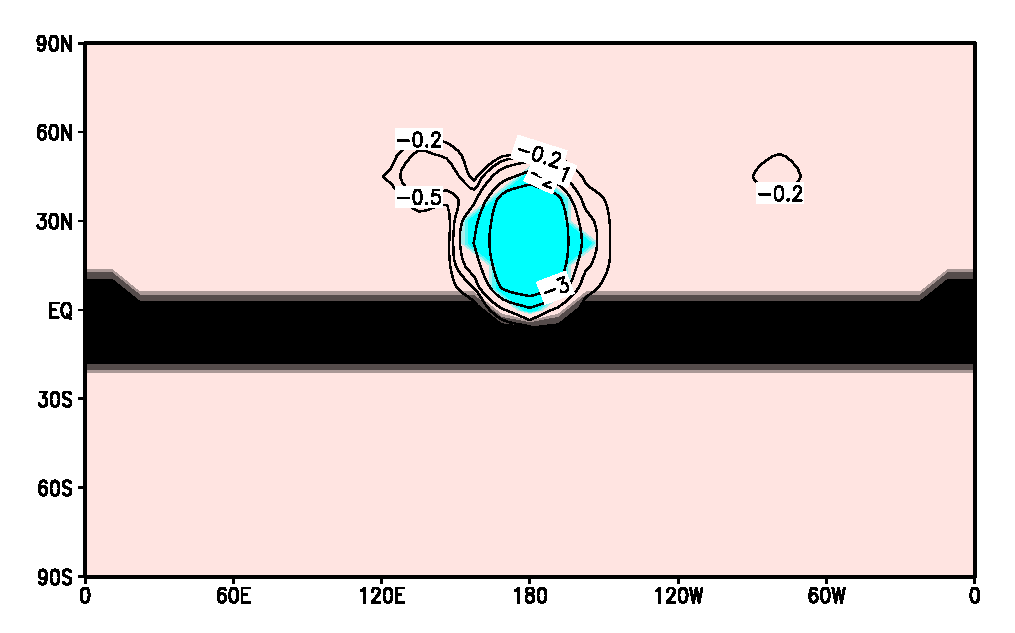
\includegraphics[width=7.cm,angle=-0,clip]{figures/map_ini1988.eps} &
   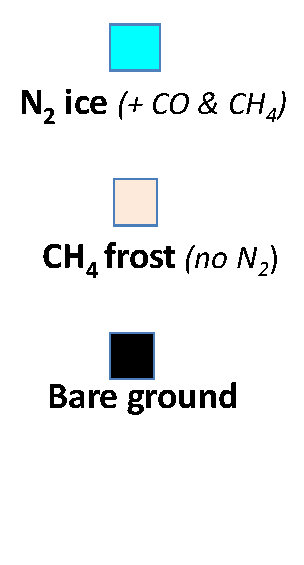
\includegraphics[width=1.4cm,angle=-0,clip]{figures/map_ini_legend.eps} &
   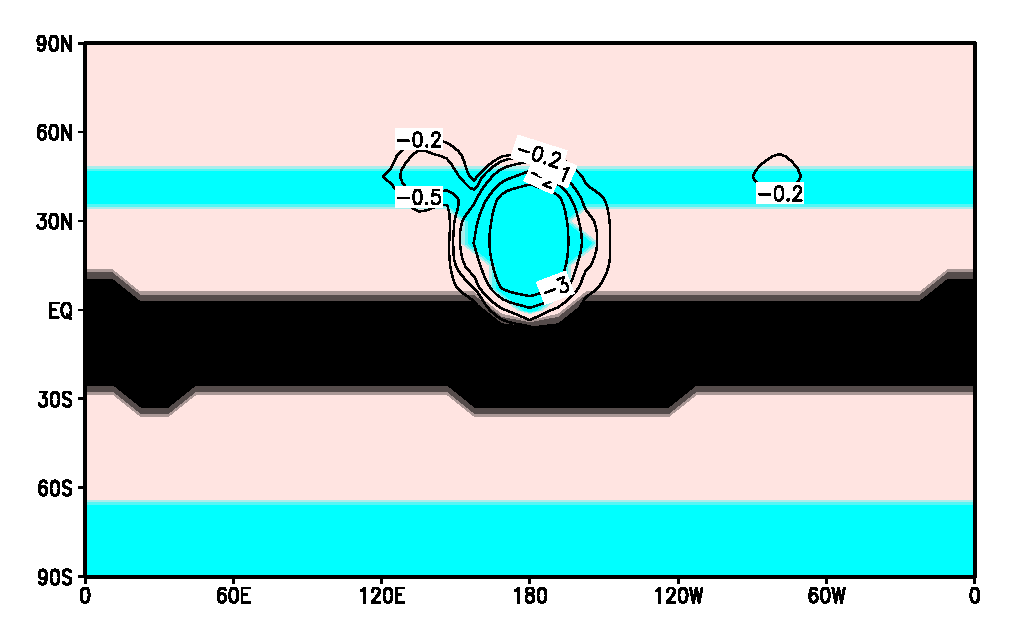
\includegraphics[width=7.cm,angle=-0,clip]{figures/map_ini2005_pole.eps}  \\
\end{tabular}
    \caption{
\label{fg:map_ini}
Maps of surface ice distribution and topography at the beginning of the reference and alternative
simulations presented in this paper. 
The black lines show the asssumed topography contours (km). 
{\bf a) }: Initial state of the reference
simulation with no N$_2$ condensation in the south polar region, in Earth year 1988. This state is
the outcome of a 40,000-Earth-years simulation performed with the reduced 2D model.
{\bf b)}: Initial state of the alternative simulation 
with N$_2$ condensation in the south polar region, in
Earth year 2005. This state is derived from the reference simulation state in 2005, with nitrogen
added between 35$^\circ$N and 48$^\circ$N and subsurface temperature poleward of 65$^\circ$S
decreased by 0.5~K. 
}
  \end{center}
\end{figure*}
%%%%%%%%%%%%%%%%%%%%%%%%%%%%%%%%%%%%%%%%%%%%%%%%%%%%%%%%%%%%%%%%%%%%%%
%%%%%%%%%%%%%%%%%%%%%%%%%%%%%%%%%%%%%%%%%%%%%%%%%%%%%%%%%%%%%%%%%%%%%%
\begin{figure*}
  \begin{center}
   \includegraphics[width=12.cm,angle=-0,clip]{figures/evol_p1215km.eps} \\
   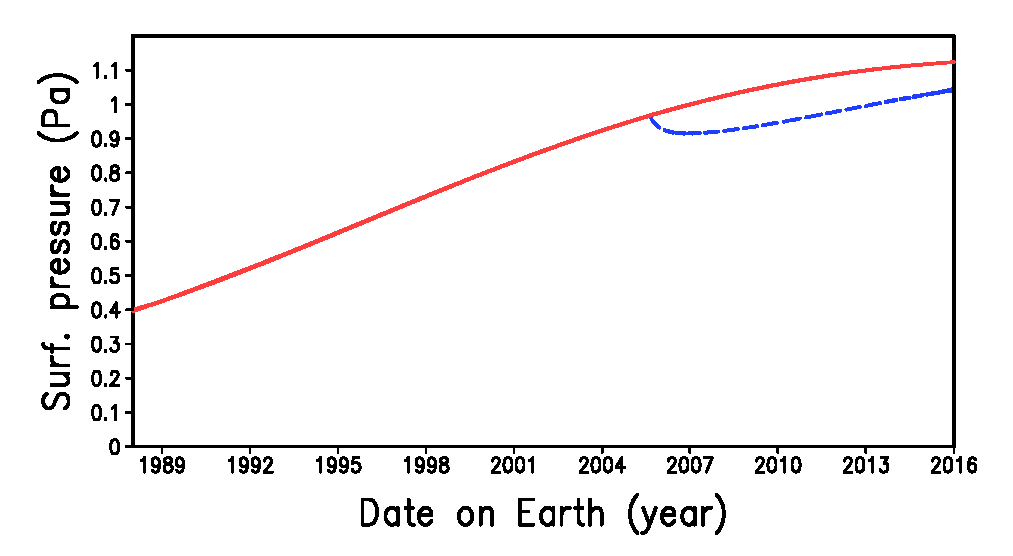
\includegraphics[width=12.cm,angle=-0,clip]{figures/evol_ps.eps} \\
    \caption{
Evolution of the pressure at $r=1215$~km from the planet center 
({\bf Top}) 
and of the global mean surface pressure 
({\bf Bottom}) 
in the reference simulation with 
no south pole N$_2$ condensation (red solid line) and in the alternative simulation with south pole
N$_2$ condensation (blue dashed line) starting at the end of 2005. The black dots with error bars show the
pressure data at  $r=1215$~km obtained by stellar occultations, as compiled by \cite{Sica:16}.
\label{fg:evol_ps}
}
  \end{center}
\end{figure*}
%%%%%%%%%%%%%%%%%%%%%%%%%%%%%%%%%%%%%%%%%%%%%%%%%%%%%%%%%%%%%%%%%%%%%%


%%%%%%%%%%%%%%%%%%%%%%%%%%%%%%%%%%%%%%%%%%%%%%%%%%%%%%%%%%%%%%%%%%%%
\section{Model results: Temperatures and winds}
%%%%%%%%%%%%%%%%%%%%%%%%%%%%%%%%%%%%%%%%%%%%%%%%%%%%%%%%%%%%%%%%%%%%
\label{sc:Tresults}

%\input {results}

\subsection{Surface temperatures and low level winds}

\subsubsection{Surface temperatures}
Fig~\ref{fg:map_ts} shows maps of surface temperatures and winds at 20~m above the surface at
various times of the day for our different simulations. The epoch corresponds 
to July 2015, the time of the New
Horizons encounter. In these simulations, surface temperatures range between 36.6 and 48~K. The
lowest values correspond to the N$_2$ frost point around 1~Pa. The highest temperatures are more
model dependent, and vary with the assumed diurnal thermal inertia
$I_{\mbox{\scriptsize day}}$.
Daytime surface temperatures
reach 57~K in GCM runs, assuming 
$I_{\mbox{\scriptsize day}}=20$~J s$^{-1/2}$ m$^{-2}$ K$^{-1}$ \citep[as reported by][]{Lell:11spitzer} 
instead of 
$I_{\mbox{\scriptsize day}}=50$~J s$^{-1/2}$ m$^{-2}$ K$^{-1}$, as assumed
in our baseline simulations.

\subsubsection{Slope winds}

On flat surfaces and where nitrogen condensation-sublimation flows are  negligible, 
wind velocities at 20~m remain well below 1~m~s$^{-1}$. In particular surface temperature gradients do
not induce significant thermal circulations.
As on Mars however, slopes can create significant downward katabatic winds resulting from the fact
that the surface is much 
colder than the atmosphere. The air close to the slopes is cooled and
tends to flow down because it is denser than the air away from the slope at the same level. 
Fig~\ref{fg:map_ts_mountain} illustrates the formation of such winds on two (hypothetical) 4-km
high, 800-km wide mountains. The wind at 20~m above the surface reaches 4~m~s$^{-1}$.
Because the atmosphere is always warmer than the surface, and because of its long radiative
timescale, the diurnal variations of surface temperature have a 
limited effect on the katabatic winds  which only increase by 20~\% during the night compared to
the day. Downward katabatic winds can also be observed on the modeled
Burney and Guest craters at 45$^\circ$N in Fig~\ref{fg:map_ts}, left column.

\subsubsection{Surface winds induced by condensation-sublimation flows}

Wind velocities larger than several meters per second can also result from 
the condensation and sublimation of nitrogen. In our reference circulation (with no condensation at
the South pole), this only occurs in the modeled ``Sputnik Planum'' area. If one assume a flat
topography (Fig~\ref{fg:map_ts}, center column), intense inward flows form during  the night
when N$_2$ condenses, and outward flows are predicted when N$_2$ sublimes during the afternoon. In
a more realistic simulation taking into account the topographic depression in Sputnik Planum
(Fig~\ref{fg:map_ts}, left column),
this effect is combined with the slope winds on the sides of the basin. During the
night, when N$_2$ condenses, both slope winds and condensation flows contribute to create winds
flowing into the modeled Sputnik Planum. During the day, however, the outward sublimation
flow is damped by the
opposite katabatic flow. 

In our alternative model (Fig~\ref{fg:map_ts}, right column),  
N$_2$ condenses in the south polar region and this sink is
balanced by the sublimation of mid-northern latitude N$_2$ deposits. This creates planetary scale
condensation flows from the northern hemisphere toward the south pole, and from the dayside toward
the nightside. 
The wind at 20~m reaches several meters per seconds over most of the planet. In both hemisphere 
its direction is affected by the Coriolis force, which prevents the atmosphere from 
flowing directly southward.  



%%%%%%%%%%%%%%%%%%%%%%%%%%%%%%%%%%%%%%%%%%%%%%%%%%%%%%%%%%%%%%%%%%%%%%
%%%%%%%%%%%%%%%%%%%%%%%%%%%%%%%%%%%%%%%%%%%%%%%%%%%%%%%%%%%%%%%%%%%%%%
\begin{figure*}
  \begin{center}
    \includegraphics[width=17.cm,angle=-0,clip]{figures/fig_tsurf.eps} 
    \caption{
\label{fg:map_ts}
Maps of surface temperature and winds at 20 meters above the surface in July 2015 at different
local times for 3 simulations: 
a) the reference simulations with no N$_2$ condensation at the south pole, 
b) The same simulation with flat topography (started from the reference run on
Juanuary 1st, 2015, and analyzed on July 14, 2015) 
c) the alternative simulation with N$_2$
condensation at the south pole. 
From top to bottom, the local time $LT$ in
the middle of the map (longitude 180$^\circ$) is 3:00, 9:00, 15:00 and 21:00,
with
$LT$~(hours)~= [longitude~($^\circ$)~- subsolar~point longitude~($^\circ$)]/15 + 12
    }%
  \end{center}
\end{figure*}
%%%%%%%%%%%%%%%%%%%%%%%%%%%%%%%%%%%%%%%%%%%%%%%%%%%%%%%%%%%%%%%%%%%%%%

%%%%%%%%%%%%%%%%%%%%%%%%%%%%%%%%%%%%%%%%%%%%%%%%%%%%%%%%%%%%%%%%%%%%%%
\begin{figure*}
  \begin{center}
\renewcommand{\arraystretch}{0.2}
\renewcommand{\tabcolsep}{-0.0cm}
\begin{tabular}[h]{ll}
%\hspace{-1cm} LT(0$^\circ$E) = 3:00 &  LT(0$^\circ$E) = 9:00 condensation \\
\hspace{-1cm}
{\bf a) } & {\bf b) } \\
\hspace{-1cm}
    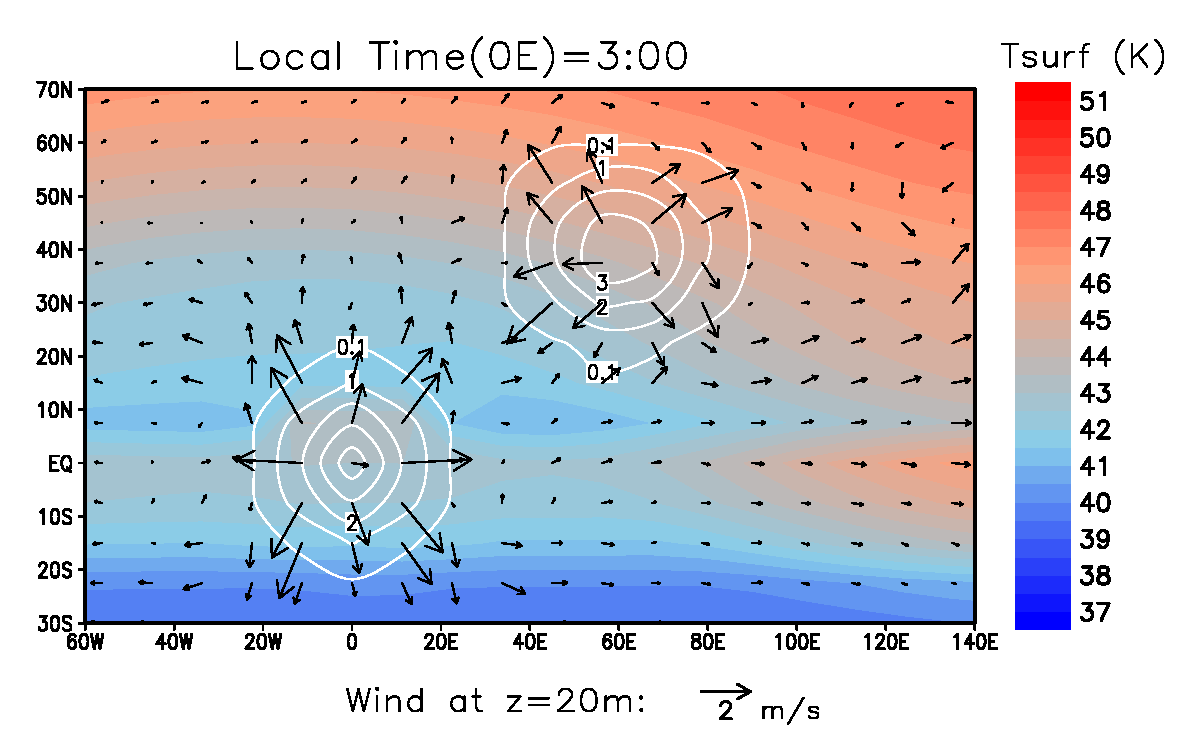
\includegraphics[height=5.5cm,angle=-0,clip]{figures/maptsurf_wind_moun2_UT3.eps} &
    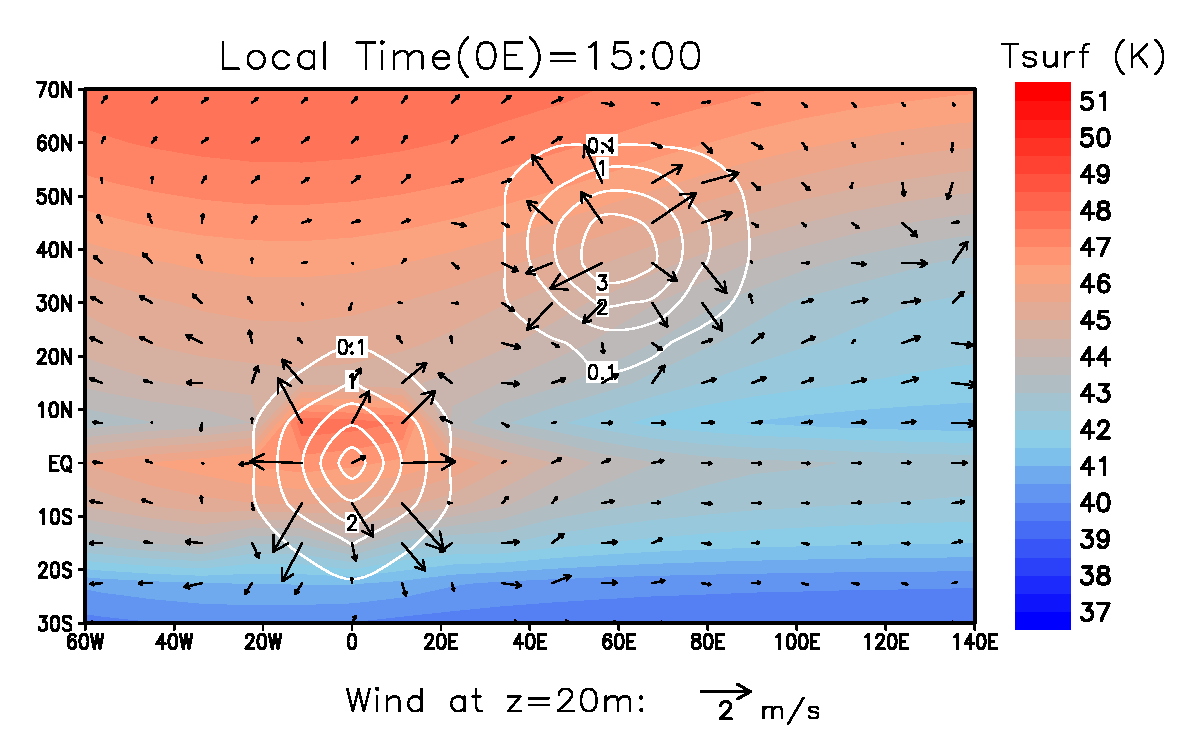
\includegraphics[height=5.5cm,angle=-0,clip]{figures/maptsurf_wind_moun2_UT15.eps}
\\
\end{tabular}
    \caption{
\label{fg:map_ts_mountain}
Maps of surface temperature and winds at 20 meters above the surface in
July 2015 in the sub-charon hemisphere, where two artificial 4000~m-high mountains has 
been added to illustrate the formation of downward slope winds on Pluto. 
The topography is shown by white contours. 
The local time at longitude 0$^\circ$E is 3:00 (nighttime) and 15:00 (daytime). 
    }%
  \end{center}
\end{figure*}
%%%%%%%%%%%%%%%%%%%%%%%%%%%%%%%%%%%%%%%%%%%%%%%%%%%%%%%%%%%%%%%%%%%%%%


\subsection{Atmospheric temperatures}

\subsubsection{Zonal-mean temperatures}

Fig.~\ref{fg:sectionT} presents the zonal-mean and global-mean atmospheric 
temperatures. As found by \cite{Toig:15}, the horizontal gradients of temperature 
are very small because of the long radiative timescale. In particular, the meridional variations in
temperatures are less than 1~K. In our reference simulation with no south pole N$_2$ condensation,
the atmospheric concentration of methane is realistic (see Section~\ref{sc:ch4_results}), and the
mean temperature profile is in acceptable agreement with available observations 
\citep{Hins:15dps,Glad:16,Dias:15}, except that above 160~km modeled temperatures are 10 to 15~K higher
than reported. The thermal structure produced in our alternative simulation with South pole N$_2$
condensation is even warmer, because of the excessive methane concentration in this
simulation, as explained in Section~\ref{fg:ch4}.

%%%%%%%%%%%%%%%%%%%%%%%%%%%%%%%%%%%%%%%%%%%%%%%%%%%%%%%%%%%%%%%%%%%%%%
\begin{figure}
  \begin{center}
\hspace*{-1cm}
   \includegraphics[width=18.cm,angle=-0,clip]{figures/fig_tempzon.eps} 
    \caption{
\label{fg:sectionT}
Zonal-mean temperatures (K) in (a) the reference
 and (c) the alternative simulations in July 2015. The central plot (b) shows 
the global mean temperature profiles.
}
  \end{center}
\end{figure}
%%%%%%%%%%%%%%%%%%%%%%%%%%%%%%%%%%%%%%%%%%%%%%%%%%%%%%%%%%%%%%%%%%%%%%




\subsubsection{Comparison with the observed REX profiles}

In Fig.~\ref{fg:hinson}, the simulated temperature profiles are compared in more details with the 
New Horizons REX radio-occultation profiles
obtained at two locations on opposite sides of Pluto.  The modeled profiles are taken at the 
same location and time, except that the ingress profile is shifted
from latitude 17.0$^\circ$S to 7.5$^\circ$N, in order to locate it just inside 
the modeled Sputnik Planum basin. 
Indeed, on the real Pluto 
the ingress profile corresponds to a location just above the southern tip of
the Sputnik Planum depression, above a surface covered by nitrogen ice. At the same coordinates in
our model, we are outside the basin and the surface is frost free. However, we found that taking into
account the low topography and N$_2$ coverage is key to understand the differences between the two
REX profiles. We plot the modeled temperature profiles as a function of  
altitude above the surface. This creates an apparent shift in temperatures (the profiles are much
more similar when shown in pressure coordinates) which contributes to
the apparent differences reported in the observations. 

Of special interest are the lowest
kilometers of the simulated ingress profiles which exhibit a low temperature layer analogous to
the bottom of the observed ingress profile. Which process creates this layer?
To better understand this behaviour, and possibly interpret
the observations, we show in Fig~\ref{fg:diuT} the diurnal evolution of the atmospheric profile in
the lowest 4~km in different modeled configurations. In the reference simulation, the atmospheric
temperature in the Spunik Planum basin varies with local time, with coldest temperatures in the
afternoon.  This results from the sublimation of nitrogen ice
when the sun heats the area, as proposed by \cite{Hins:15agu}. In fact,
the volume of gas involved in the condensation-sublimation cycle is considerable in our
model. Fig.~\ref{fg:diuN2} shows the nitrogen ice budget in the modeled Sputnik Planum basin at
7.5$^\circ$N and 45$^\circ$N. At this last position, about 230~g~m$^{-2}$ of ice sublimates every
Pluto day
in 2015. As shown on the right axis of Fig.~\ref{fg:diuN2}, this corresponds to more than
2500~m$^{3}$ of N$_2$ gas per square meter. 
At 7.5$^\circ$N, the solar flux is weaker in 2015 and the daily
N$_2$ ice budget corresponds to a net gain in N$_2$ ice (net condensation). Nevertheless, every
afternoon the equivalent of 800~m$^{3}$ per square meters is injected into the atmosphere.
Moreover, in the GCM the large amount of cold N$_2$ gas produced at higher latitude (where the
insolation is higher) is spread throughout the basin in the lowest kilometers.
In fact, in the alternative simulation this process contributes 
to increasing the amount of cold air present in the modeled Spunik Planum basin
(Fig.~\ref{fg:diuT}b), 
%because of the additional 
adding the
freshly-sublimed cold N$_2$ gas
transported from the N$_2$ ice belt at 35$^\circ$N (as seen on Fig.~\ref{fg:map_ts}, right
column, local time 15:00 and 21:00). 

Interestingly, as shown in Fig.~\ref{fg:diuT}c, a simulation performed 
without taking into account the topographic depression
in the modeled Spunik-planum does not create a significant cold layer.
Two facts explain that. First, the freshly-sublimed N$_2$ gas is efficiently 
transported away as discussed above (and as seen on Fig.~\ref{fg:map_ts}, mid-column).  
Second, in an atmosphere with radiative timescale as long as Pluto,  
in a local topographic depression the temperature lapse rate is not as steep as on average
because temperatures tend to be homogeneous at a given pressure level. This is illustrated
on Fig.~\ref{fg:diuT}d which shows the temperatures at the bottom of the basin 
in a simulation with N$_2$ condensation and
sublimation completely switched off. Without N$_2$ sublimation, the air is not as cold 
as in the reference simulation, but at a given altitude above the surface, 
temperatures in the basin remain 5 to 10~K below what they would have been outside (compare
Fig.~\ref{fg:diuT}c and Fig~\ref{fg:diuT}d). 






%%%%%%%%%%%%%%%%%%%%%%%%%%%%%%%%%%%%%%%%%%%%%%%%%%%%%%%%%%%%%%%%%%%%%%
\begin{figure}
  \begin{center}
   \includegraphics[width=17.cm,angle=-0,clip]{figures/fig_hinson.eps} \\
    \caption{
\label{fg:hinson}
Comparison of the two temperature profiles retrieved by the New Horizons REX experiment 
\citep{Hins:15dps,Glad:16} 
at 193.5$^\circ$E, 17.0$^\circ$S and Local time 16:31 ({\bf red}) and 15.7$^\circ$E,
15.1$^\circ$N and Local time 04:42 ({\bf blue}) with GCM results. 
The model data are taken at the same
location and time, except for the profile at latitude 17.0$^\circ$S which is shifted to 7.5$^\circ$N
in order to locate it just within the modeled Sputnik Planum basin filled with $N_2$ ice, as it is the case in
reality (see text).  
}
  \end{center}
\end{figure}
%%%%%%%%%%%%%%%%%%%%%%%%%%%%%%%%%%%%%%%%%%%%%%%%%%%%%%%%%%%%%%%%%%%%%%


%%%%%%%%%%%%%%%%%%%%%%%%%%%%%%%%%%%%%%%%%%%%%%%%%%%%%%%%%%%%%%%%%%%%%%
\begin{figure}
  \begin{center}
\renewcommand{\arraystretch}{0.2}
\begin{tabular}[h]{cc}
\hspace{-2.cm}
 a) {\bf Reference} & b) {\bf With South Pole N$_2$ condensation} \\
\hspace{-2.cm}
   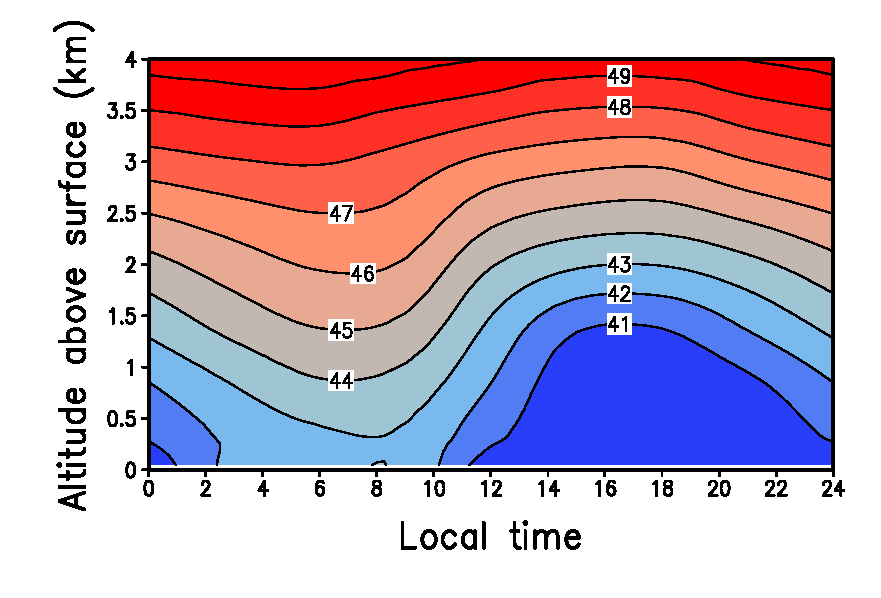
\includegraphics[width=8.cm,angle=-0,clip]{figures/diuT.eps} &
   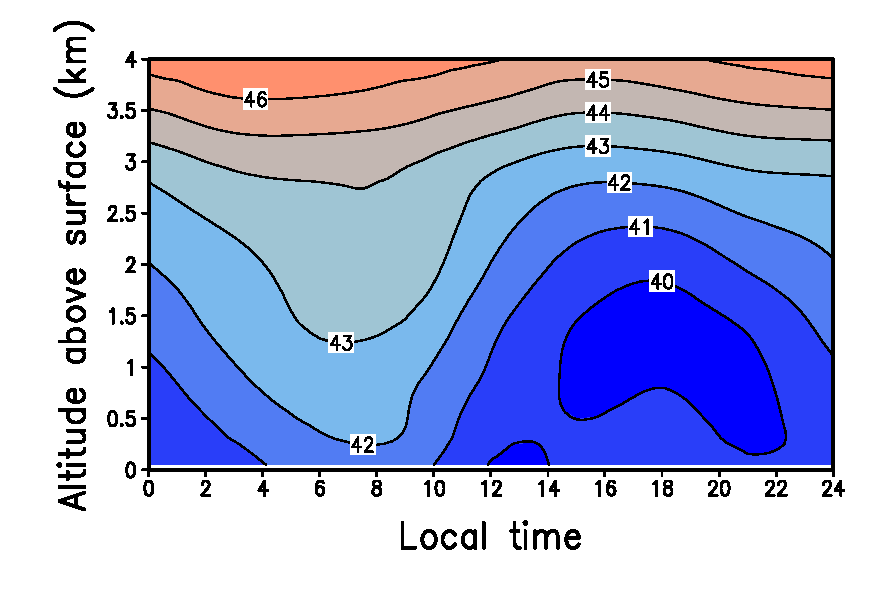
\includegraphics[width=8.cm,angle=-0,clip]{figures/diuT_pole.eps} \\
\hspace{-2.cm}
c) {\bf Flat topography} & 
d) {\bf No N$_2$ condensation/sublimation} \\
\hspace{-2.cm}
   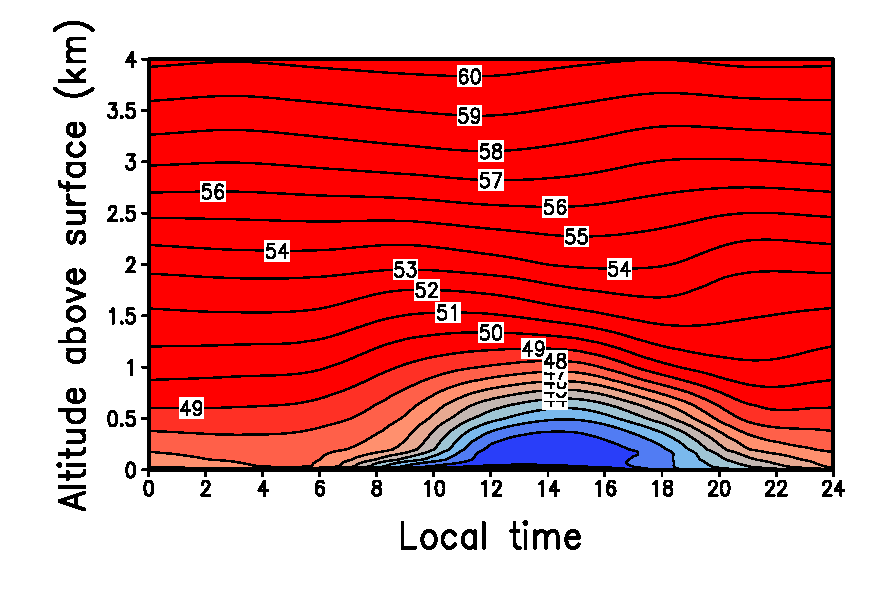
\includegraphics[width=8.cm,angle=-0,clip]{figures/diuT_flat.eps} &
   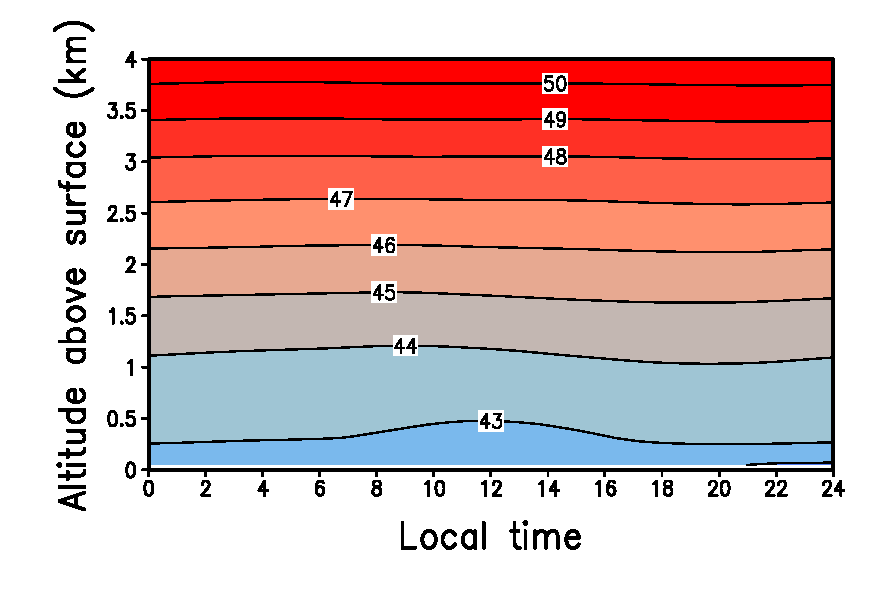
\includegraphics[width=8.cm,angle=-0,clip]{figures/diuT_nocon.eps} \\ 
\end{tabular}
    \caption{
\label{fg:diuT}
Diurnal variations of atmospheric temperature in the lower atmosphere at 
193.5$^\circ$E-7.5$^\circ$N (at the bottom of the modeled Sputnik Planum basin) 
for (a) the reference simulation
(without South Pole N$_2$ condensation), (b) the alternative simulation (with South Pole N$_2$
condensation), (c) a version of the reference simulation with a flat topography, and
(d) No N$_2$ condensation/sublimation at all on the planet.
The simulations with flat topography and No N$_2$ condensation/sublimation were 
started from the reference run initial state on January 1st, 2015,
and analyzed on July 14, 2015.
}
  \end{center}
\end{figure}
%%%%%%%%%%%%%%%%%%%%%%%%%%%%%%%%%%%%%%%%%%%%%%%%%%%%%%%%%%%%%%%%%%%%%%

%%%%%%%%%%%%%%%%%%%%%%%%%%%%%%%%%%%%%%%%%%%%%%%%%%%%%%%%%%%%%%%%%%%%%%
\begin{figure}
  \begin{center}
\renewcommand{\arraystretch}{0.2}
\begin{tabular}[h]{cc}
\hspace{-2.cm}
  a) Latitude: 7.5$^\circ$N  & b) Latitude: 45$^\circ$N  \\
\hspace{-2.cm}
   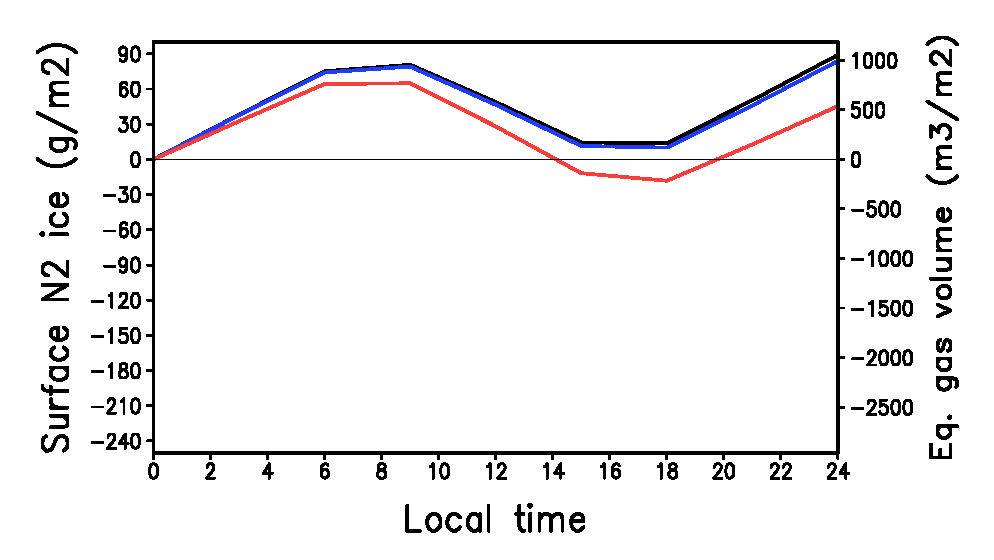
\includegraphics[width=8.cm,angle=-0,clip]{figures/diuN2_7.eps} &
   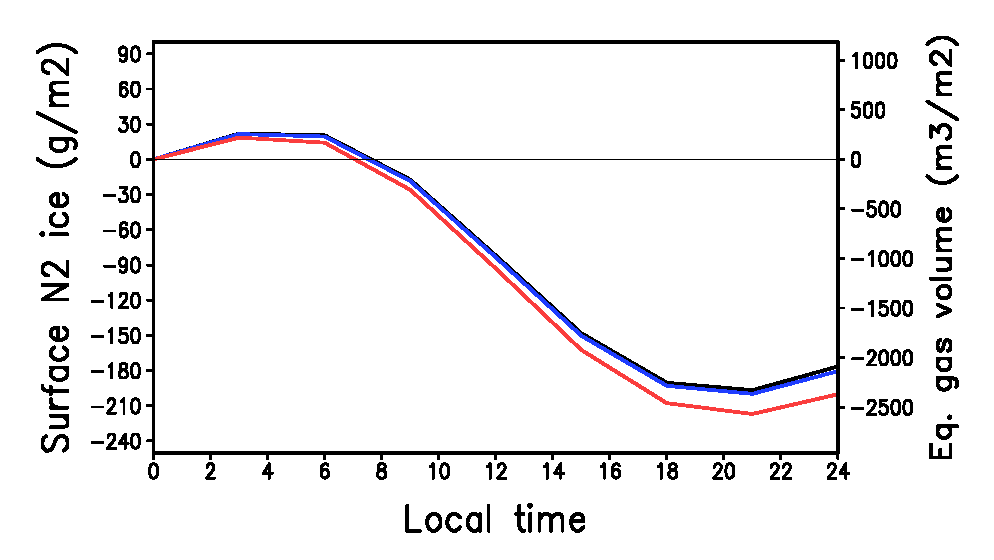
\includegraphics[width=8.cm,angle=-0,clip]{figures/diuN2_45.eps} \\
\end{tabular}
    \caption{
\label{fg:diuN2}
Diurnal variation of the surface N$_2$ ice loading at two different latitudes in the modeled
``Sputnik Planum'' basin in July 2015. 
The right axis illustrates the corresponding volume of N$_2$ gas, assuming
a pressure of 1~Pa and a temperature of 40~K. The different line colours correspond to different
kinds of simulations: reference (blue), alternative with South pole N$_2$ condensation (black, partly
hidden by the blue line), and with a flat topography (red). The curves do not loop (i.e. the values
at 24:00 differ from the values at 0:00) because every Pluto day the integrated surface budget
corresponds
to a net gain of N$_2$ ice by condensation at 7.5$^\circ$N and a net loss by sublimation at
45$^\circ$N, where the incident solar flux is stronger than at 7.5$^\circ$N.
}
  \end{center}
\end{figure}

%%%%%%%%%%%%%%%%%%%%%%%%%%%%%%%%%%%%%%%%%%%%%%%%%%%%%%%%%%%%%%%%%%%%%%

\subsubsection{Thermal tides and waves}


Stellar occultations have shown that vertical profiles of 
density fluctuations in the atmosphere of Pluto
often exhibit wave-like structure \citep[e.g.][]{Sica:03,Pers:08} with an amplitude of a few
percent and vertical wavelengths of a few kilometers.
On the basis of theoretical calculations, \cite{Toig:10} suggested that
such waves could correspond to the tidal response of Pluto’s atmosphere 
to solar-induced sublimation ‘‘breathing” from N$_2$ frost patches. 
Here we briefly examine 
the type of wavelike structure present in the temperature profiles generated by our 
GCM. Note, however, that the horizontal and vertical resolution used in the GCM
simulations is unlikely to capture waves with vertical wavelengths smaller than
$\sim20$~km. 

Fig.~\ref{fg:tide}a presents the 4-sols evolution of the difference between 
instantaneous temperatures and 1-Pluto-day gliding averages at
0$^\circ$E - 0$^\circ$N in our reference simulation. The observed temperature excursions 
are lower than 0.2~K.  Nevertheless, they are characteristic of upward atmospheric thermal tides, 
with, below 80~km, diurnal, wavenumber=1 thermal tides with a vertical wavelength around
20~km and a downward phase velocity. Above 150~km, semi-diurnal wavenumber=2 tide with much
longer vertical wavelengths start to dominate. As predicted by \cite{Toig:10}, the source of
the tides is the diurnal N$_2$ condensation-sublimation cycle of the N$_2$ ice: 
Tidal amplitude are 4-times weaker if N$_2$ 
condensation-sublimation processes are switched off. 

Fig.~\ref{fg:tide}b presents the same anomaly plot in the alternative simulations with N$_2$
condensation occuring at the south pole. The amplitude of the waves are significantly larger,
reaching more than $\pm$1~K around 120~km. However, a careful examination of
Fig.~\ref{fg:tide}b reveals that the period of the stronger waves is not 1 nor 0.5~Pluto day.
These are not thermal tides: the same waves are present in simulations forced by a
diurnally-averaged insolation (no diurnal cycle and no tides). These waves appear to be
barotropic waves produced by a southern polar jet, as described in
Section~\ref{fg:wind2}.



%%%%%%%%%%%%%%%%%%%%%%%%%%%%%%%%%%%%%%%%%%%%%%%%%%%%%%%%%%%%%%%%%%%%%%
\begin{figure}
  \begin{center}
\renewcommand{\arraystretch}{0.2}
\begin{tabular}[h]{cc}
\hspace{-2.cm}
   a) No South Pole N$_2$ condensation & b) With South Pole N$_2$ condensation \\
\hspace{-2.cm}
   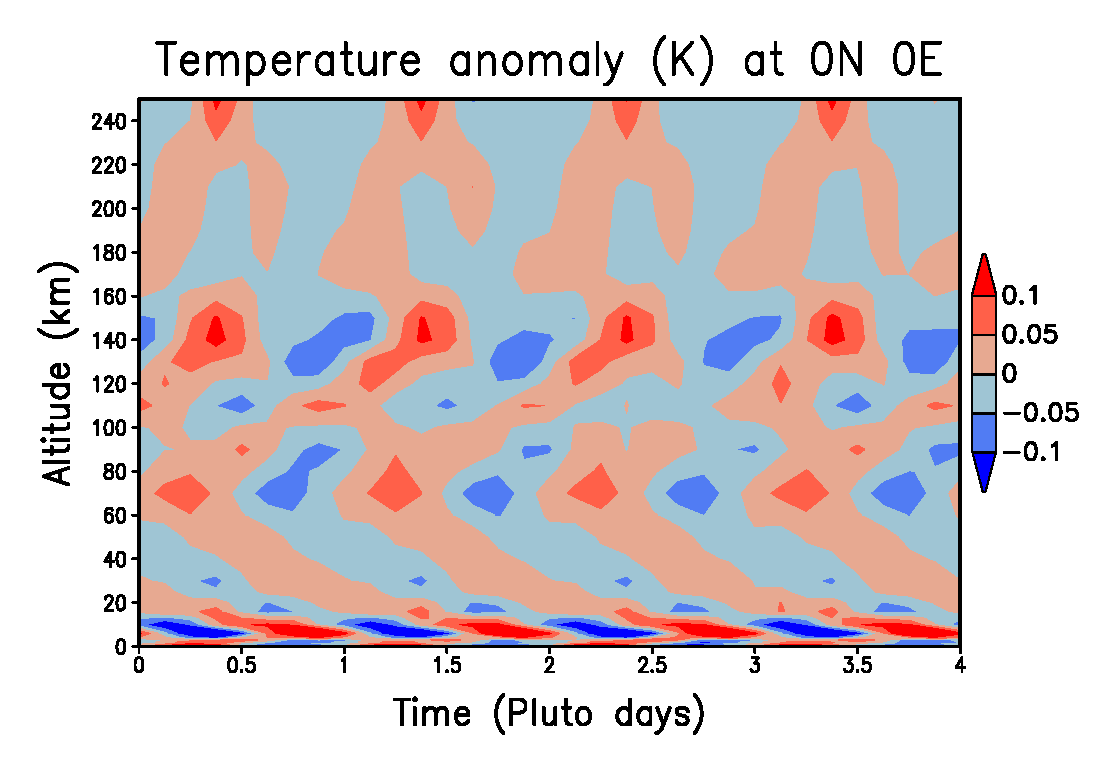
\includegraphics[width=8.cm,angle=-0,clip]{figures/tide_T_0E_0N.eps} &
   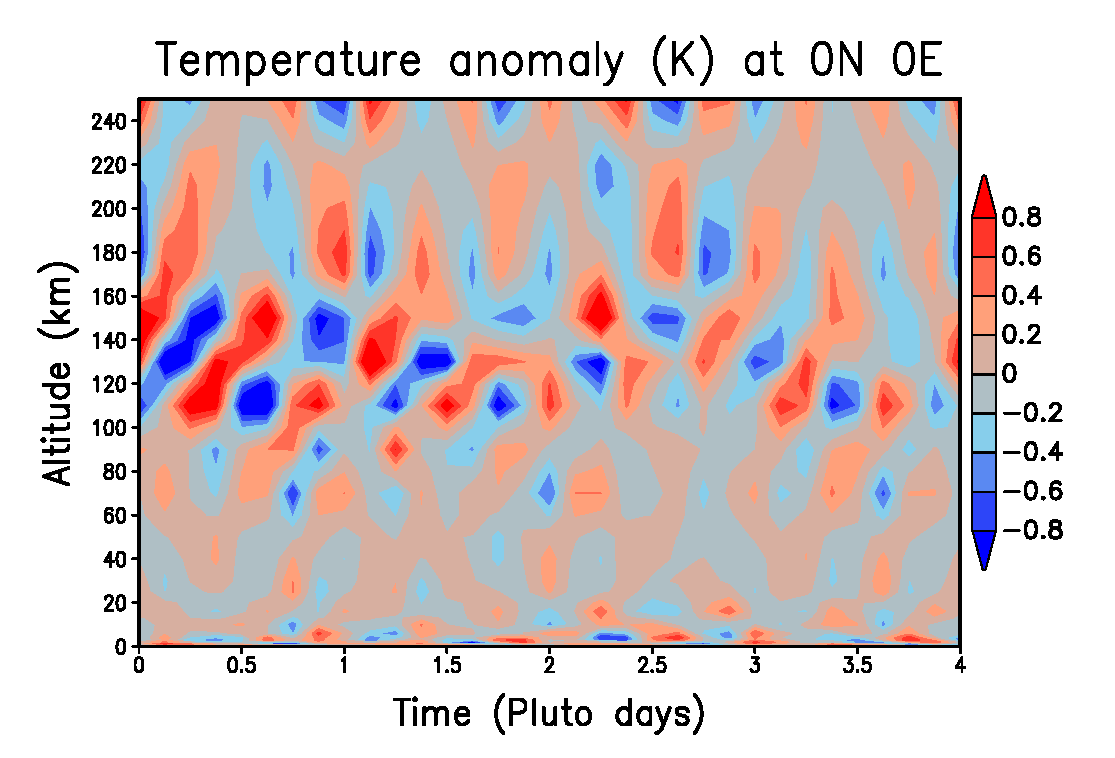
\includegraphics[width=8.cm,angle=-0,clip]{figures/tide_T_0E_0N_pole2.eps} \\
\end{tabular}
    \caption{
\label{fg:tide}
Temperature anomaly (difference between instantaneous value and diurnal average) at  
0$^\circ$E - 0$^\circ$N in the reference and alternative simulations in July 2015. Thermal tides are
clearly visible in the reference simulation, whereas the alternative simulation is characterized by
atmospheric barotropic waves (see text). 
}
  \end{center}
\end{figure}
%%%%%%%%%%%%%%%%%%%%%%%%%%%%%%%%%%%%%%%%%%%%%%%%%%%%%%%%%%%%%%%%%%%%%%







%%%%%%%%%%%%%%%%%%%%%%%%%%%%%%%%%%%%%%%%%%%%%%%%%%%%%%%%%%%%%%%%%%%%%%
\subsection{Atmospheric circulation and waves}
%%%%%%%%%%%%%%%%%%%%%%%%%%%%%%%%%%%%%%%%%%%%%%%%%%%%%%%%%%%%%%%%%%%%%%

Fig.~\ref{fg:section_wind} shows cross-sections of the average zonal (west-east) and
meridional (south-north) winds in our two baseline simulations. 

\subsubsection{Reference Case without N$_2$ condensation at the south pole,}

In the reference case with no condensation-flow induced by N$_2$ condensation at the south pole, 
the circulation is relatively weak with slow retrograde zonal
winds in the northern hemisphere and the equatorial regions
(Fig.~\ref{fg:section_wind}a).  This circulation remains unchanged
with a flat topography, no diurnal cycle, or when N$_2$ condensation and
sublimation processes are switched off. It 
can be explained by the north-south latitudinal gradient of solar heating rates. 
It induces a very small temperature contrast between the spring and fall hemisphere and, in 
turn, forces weak zonal winds corresponding to the thermal wind balance. 
Consistently, the weak meridional
circulation (Fig.~\ref{fg:section_wind}c) is characterized by a cell 
centered at the equator (where the Coriolis force is null) 
between 80 and 140~km, with the upper branch flowing from the sunlit hemisphere toward
the polar night hemisphere. 


\subsubsection{Alternative case with N$_2$ condensation at the south pole,}

\label{fg:wind2}

The circulation is profoundly influenced by the North-South condensation flow if N$_2$
condenses in the South polar regions. 

If N$_2$ ice deposits were covering the entire northern polar regions (which is not
observed) and the southern hemisphere condensation much more intense, 
the condensation flow would be very strong. 
As obtained in some of our past simulations (not
shown) and as reported in some scenarios analysed by \cite{Toig:15} (see their Fig. 11 
and~18), the meridional
circulation would be characterized by a global flow from the northern hemisphere to the
southern hemisphere. In such conditions, the zonal circulation is characterized by a
global ``retro-superrotation'' with retrograde winds at most latitude. Such winds result
from the conservation of angular momentum of the air particles as they flow from the sunlit
pole to the polar night above the equator, where they are farther from the 
rotation axis than where they started from. 

In our simulations however, the North-South condensation flow remains limited compared to
this extreme case. We consider that this is in better agreement with the observations 
because 1)~outside Sputnik Planum the N$_2$ ice frost deposits are limited to patches around
45-60$^{\circ}$N \citep{Grun:16}, and 2)~because the south pole 
N$_2$ condensation cannot be very intense in 2015 since Pluto's surface pressure has been
increasing in recent years. 

With the realistic assumptions made in our ``alternative'' simulation, the meridional
circulation remains weak (Fig.~\ref{fg:section_wind}d) 
and strongly modulated by waves (see below). The overall transport
pattern is southward, as revealed when analysing tracer transport \citep{Bert:16ica}. 

The zonal wind is charaterized by an intense prograde jet-stream poleward of 40$^\circ$S and
a prograde superrotation at most other latitudes (Fig.~\ref{fg:section_wind}c). 
The high-latitude jet is a 
classical feature of terrestrial atmospheres, and likely result here from the
poleward condensation flow and the conservation of angular momentum. Superrotation is
more surprising. It is observed on Venus and Titan and has been the subject of many studies
\citep[see, e.g. ][and references therein]{Lebo:10}. In these cases, superrotation is
considered to primarily result from the so-called Gierasch-Rossow-Williams mechanism
\citep[from][]{Gier:75,Ross:79}. In this mechanism, waves, possibly generated  
by barotropic instabilities from the high-latitude jets, redistribute angular momentum
equatorward. Preliminary analysis suggest that this is what is happening in our simulation. 
A study of the variations of the high-latitude jet show that it is subject to
instabilities that create a wavenumber~1 wave that propagates eastward with a 0.5-0.8~Pluto day
period. At 60$^{\circ}$N, such waves are clearly visible at an altitude of 140~km 
in the temperature and meridional wind fields (Fig.~\ref{fg:waves}b and
\ref{fg:waves}d). In~Fig.~\ref{fg:waves}c, the extension of this wave is
mapped by plotting the meridional wind variability as a function of latitude and
height. One can see that it propagates to all latitudes, and notably to the equator,
where the signature in the thermal field dominates the temperature variability 
(Fig.~\ref{fg:waves}a). Similar results are obtained in model runs 
without a diurnal cycle or with a flat topography.

In addition to the wind predictions published by \cite{Toig:15}, already  discussed, our
results can be compared with the results from the other Pluto GCM proposed by 
\cite{Zalu:13}
and \cite{Zalu:16}. The comparison with \cite{Zalu:13} is difficult to achieve
because this version of their GCM did not yet include nitrogen condensation and because their
modeled thermal structure was very different than what was observed on Pluto by New Horizons. In
fact the updated version presented by \cite{Zalu:16} yielded completely different results. Her 
``Case 1'', in which a surface pressure of 0.8~Pa and 1\% of CH$_4$ is assumed, can be compared
to our simulations. The zonal wind structure ressemble our reference simulation, suggesting that,
for unknown reasons, the condensation flow is weak in this GCM in spite of the fact that Pluto is
assumed to be covered by nitrogen ice.

%%%%%%%%%%%%%%%%%%%%%%%%%%%%%%%%%%%%%%%%%%%%%%%%%%%%%%%%%%%%%%%%%%%%%%
\begin{figure}
  \begin{center}
\renewcommand{\arraystretch}{0.2}
\begin{tabular}[h]{cc}
\hspace{-2.cm}
   {\bf REF: No South Pole N$_2$ condensation} & {\bf ALT: With South Pole N$_2$ condensation} \\
\hspace{-2.cm}
   {a) Mean zonal wind (m~s$^{-1}$) } & {b) Mean zonal wind (m~s$^{-1}$) } \\
\hspace{-2.cm}
   \includegraphics[width=8.cm,angle=-0,clip]{figures/sectionU.eps} &
   \includegraphics[width=8.cm,angle=-0,clip]{figures/sectionU_pole.eps} \\
\hspace{-2.cm}
   {c) Mean meridional wind (m~s$^{-1}$) } & {d) Mean meridional wind (m~s$^{-1}$) } \\
\hspace{-2.cm}
   \includegraphics[width=8.cm,angle=-0,clip]{figures/sectionV.eps} &
   \includegraphics[width=8.cm,angle=-0,clip]{figures/sectionV_pole.eps} \\
\end{tabular}
    \caption{
\label{fg:section_wind}
Zonal-mean zonal and meridional winds (m~s$^{-1}$) in the reference and alternative 
simulations in July 2015. 
}
  \end{center}
\end{figure}
%%%%%%%%%%%%%%%%%%%%%%%%%%%%%%%%%%%%%%%%%%%%%%%%%%%%%%%%%%%%%%%%%%%%%%


%%%%%%%%%%%%%%%%%%%%%%%%%%%%%%%%%%%%%%%%%%%%%%%%%%%%%%%%%%%%%%%%%%%%%%
\begin{figure}
  \begin{center}
\begin{tabular}[h]{ll}
\hspace{-2.cm} {\bf a)}  & {\bf b)} \\
\hspace{-2.cm}
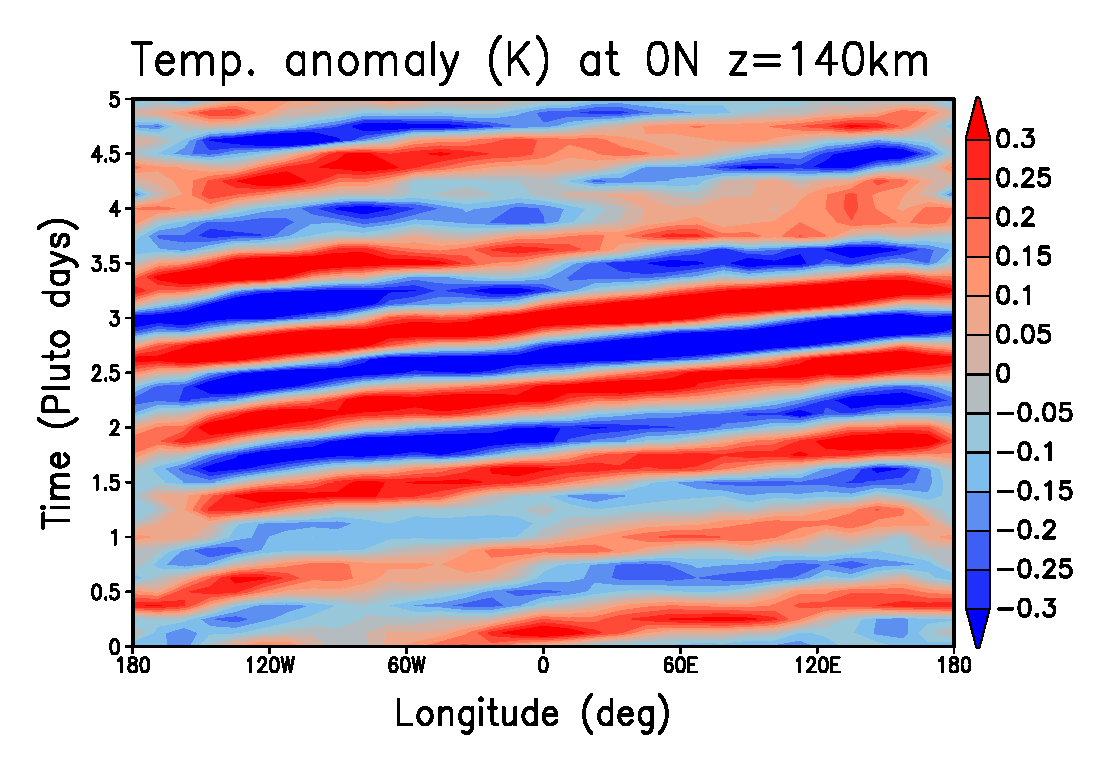
\includegraphics[width=8.cm,angle=-0,clip]{figures/wave_T_0N_140km.eps} &
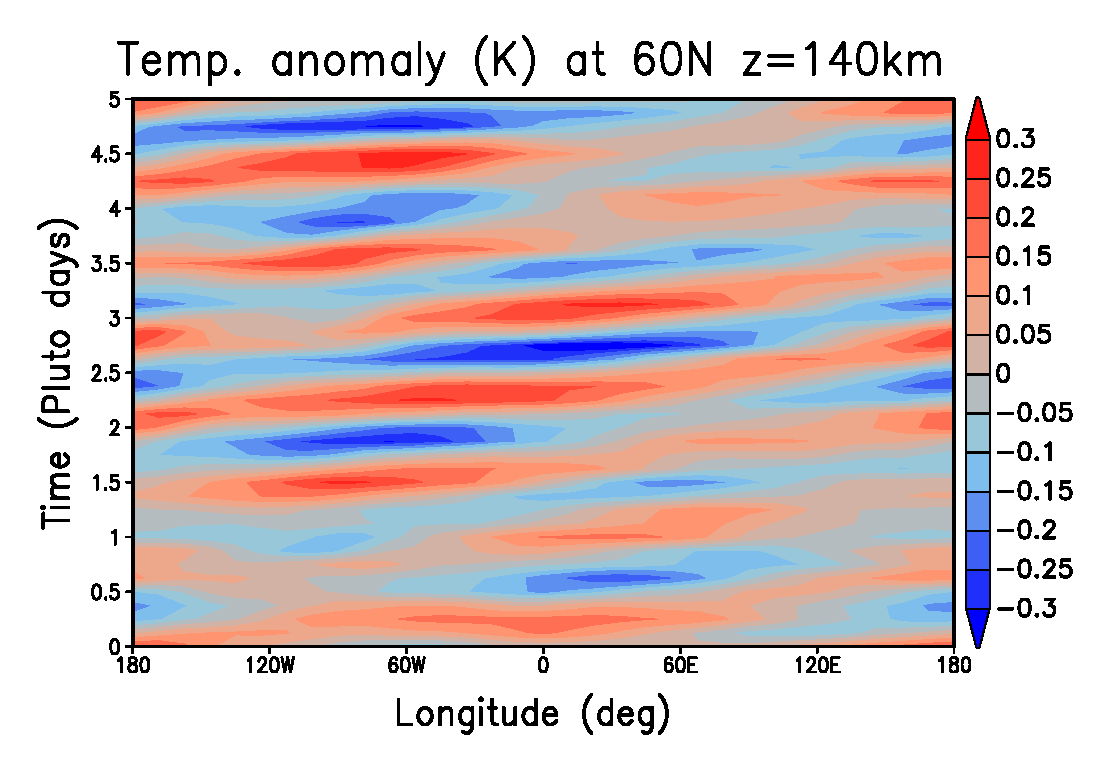
\includegraphics[width=8.cm,angle=-0,clip]{figures/wave_T_60N_140km.eps} \\
\hspace{-2.cm} {\bf c)} & {\bf d)} \\
\hspace{-2.cm}
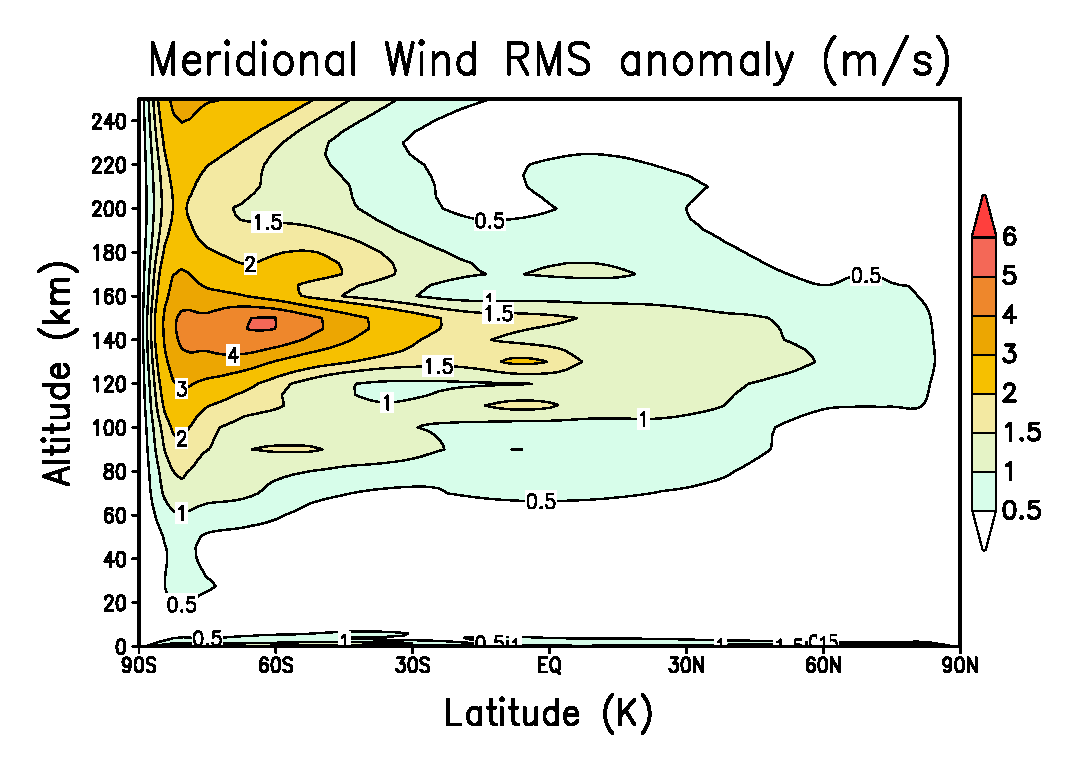
\includegraphics[width=8.cm,angle=-0,clip]{figures/rms_v_pole.eps} &
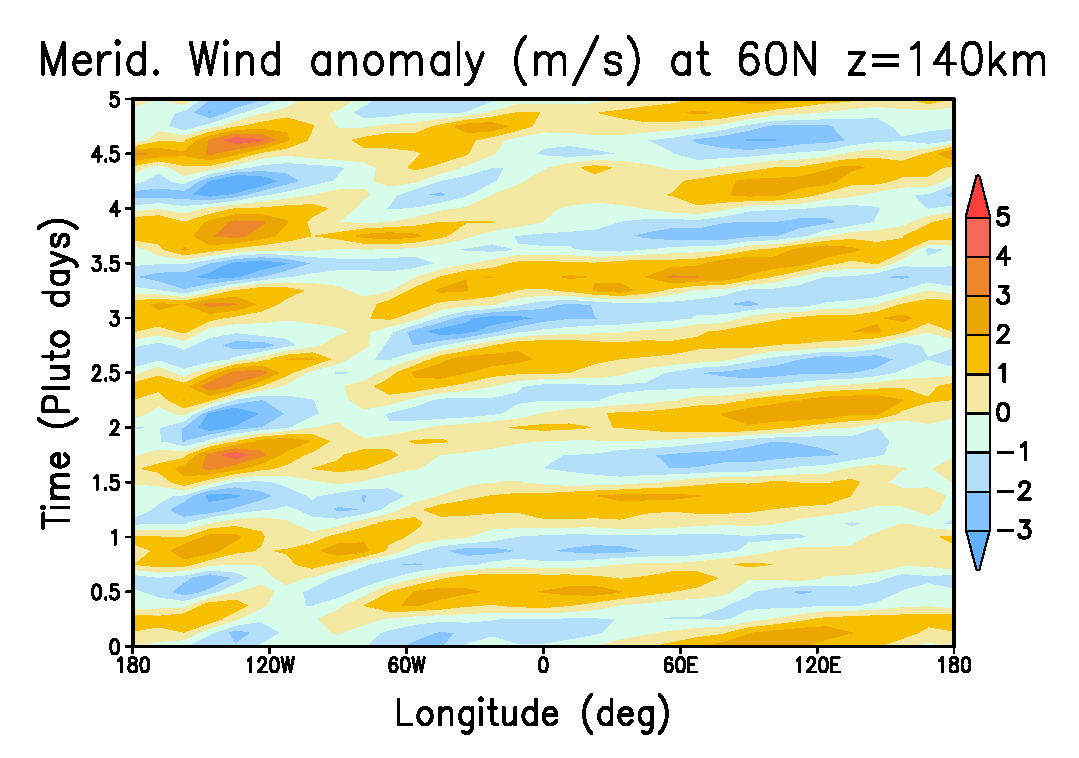
\includegraphics[width=8.cm,angle=-0,clip]{figures/wave_V_60N_140km.eps} \\
\end{tabular}
    \caption{
\label{fg:waves}
Characteristics of the barotropic waves present in the simulations with South Pole N$_2$ condensation
inducing a condensation flow. {\bf a)} H\"ovmoller diagram of the temperature anomaly (difference between
the local and the zonal-mean temperature) at 0$^\circ$N. {\bf b)} Same at 60$^\circ$N.
{\bf c)} Zonal average of the root-mean-square standard deviation of the local 
 meridional wind from the zonal-averaged meridional wind.
{\bf d)}  H\"ovmoller diagram of the meridional wind anomaly (difference between
the local and the zonal-mean wind, in m~s$^{-1}$) at 0$^\circ$N. 
}
  \end{center}
\end{figure}
%%%%%%%%%%%%%%%%%%%%%%%%%%%%%%%%%%%%%%%%%%%%%%%%%%%%%%%%%%%%%%%%%%%%%%



%%%%%%%%%%%%%%%%%%%%%%%%%%%%%%%%%%%%%%%%%%%%%%%%%%%%%%%%%%%%%%%%%%%%
\section{Model results: CH$_4$ and CO cycles }
%%%%%%%%%%%%%%%%%%%%%%%%%%%%%%%%%%%%%%%%%%%%%%%%%%%%%%%%%%%%%%%%%%%%
\label{sc:ch4_co_results}



\subsection{Evolution and distribution of gaseous CH$_4$}
%%%%%%%%%%%%%%%%%%%%%%%%%%%%%%%%%%%%%%%%%%%%%%%%%%%%%%%%%

\label{sc:ch4_results}


Fig.~\ref{fg:ch4} shows the global-mean mixing ratio of methane 
(determined from the ratio of CH$_4$ and N$_2$
column densities) 
in our baseline simulations, and how this ratio varies over time.
Fig.~\ref{fg:ch4}c shows the evolution of the global-mean mixing ratio of methane.
The three red curves correspond to reference simulations (without
poleward condensation flow) with methane volume mixing ratio 
inialized at 0.1\%, 0.5\% and 1\% in 1988.
One can see that in 2015 the results are still sensitive to the initialization, although
the three simulations clearly converge toward a global mean value near 0.5~\%.
Fig.~\ref{fg:ch4}a and~b present the zonal-mean methane abundances as a function of latitude and
altitude in 2010 
\citep[mid-point between the 2008 and 2012 observations by][]{Lell:15} and 2015 (New
Horizons). These figures show that methane is not homogeneously distributed, notably
because the high latitude deposits are increasingly heated and sublimed as the sub-solar
point moves northward with time. As a result methane tends to be enriched in the
lower atmosphere at high northern latitudes compared to the rest of the planet, but
is otherwise vertically well mixed and near 0.5\% at most altitudes. This is
consistent with the observation analysis of \cite{Lell:15} who concluded that their 
data ``imply a roughly uniform mixing ratio in at least the first 22$-$27 km of the 
atmosphere'', and that  ``high concentrations of low-temperature methane near the
surface can be ruled out''. To compare with Earth-based near-infrared observations, 
one must nevertheless take into account the fact that such observations are biased
toward the methane column near the sub-Earth-subsolar points for geometrical reason
(Pluto is a sphere) and because this is where the insolation is maximum. 
Taking into account that the sub-Earth and subsolar points are always very close,
we can estimate the apparent mixing ratio as seen from the Earth by 
performing an average of the local column mixing ratio weighted by the square of the
cosine of the solar zenith angle. The apparent mixing ratio for the reference simulations
started with 0.5~\%~CH$_4$ is shown in green on Fig.~\ref{fg:ch4}c. The difference with
the global-mean value remain small and has only become significant
 recently with the local increase of methane above the North pole. 

On the same Figure~\ref{fg:ch4}c, 
the blue dashed curve shows the evolution of the global-mean methane
in the alternative scenario (with N$_2$ condensing at the south pole) starting in 2005.
Fig.~\ref{fg:ch4}d show the corresponding methane abundances as a function of latitude and
altitude in 2015. 
One can see that the methane content is larger and still increasing in this simulation.
This results from the stronger near-surface winds induced by the condensation flow, and
the fact that the near-surface mixing is directly proportional to the horizontal wind as
formalized in Equation~\ref{eq:sflux} presented in Section~\ref{sc:pbl}. 









%%%%%%%%%%%%%%%%%%%%%%%%%%%%%%%%%%%%%%%%%%%%%%%%%%%%%%%%%%%%%%%%%%%%%
\begin{figure}
  \begin{center}
\renewcommand{\arraystretch}{0.2}
\begin{tabular}[h]{cc}
\hspace{-1.cm}
{\bf a)  REF: CH$_4$ vol. mixing ratio in 2010 } &
{\bf b) REF: CH$_4$ vol. mixing ratio in 2015 } \\
\hspace{-1.cm}
   \includegraphics[height=5.cm,angle=-0,clip]{figures/section_ch4_2010.eps} &
   \includegraphics[height=5.cm,angle=-0,clip]{figures/section_ch4_2015.eps} \\
\hspace{-1.cm}
 Latitude & Latitude \\
\vspace{0.5cm} \\
\hspace{-1.cm}
{\bf c) Evolution of mean CH$_4$ vol. mixing ratio} &
{\bf d) ALT: CH$_4$ in 2015 with south pole N$_2$ condensation} \\
\hspace{-1.cm}
   \includegraphics[height=5.cm,angle=-0,clip]{figures/evol_ch4.eps} &
   \includegraphics[height=5.cm,angle=-0,clip]{figures/section_ch4_pole_2015.eps} \\
\hspace{-1.cm}
 Date on Earth (year) & Latitude \\
\end{tabular}
    \caption{
\label{fg:ch4}
{\bf a) - b)}: Zonal mean methane volume mixing ratio (\%) in the reference simulation 
(without south pole N$_2$ condensation and [CH$_4$] initially at 0.5\% in 1988) 
in 2010 and 2015. 
{\bf c)}: Evolution of the mean volume mixing ratio: 
globally averaged with different initialization (red), the apparent mixing ratio
 as seen from the Earth (green, see text) 
and in the alternative simulation with south pole N$_2$ condensation started in 2005 (dashed blue).
{\bf d)}: Zonal mean methane volume mixing ratio (\%) in the alternative simulation
(with south pole N$_2$ condensation) in 2015. 
}
  \end{center}
\end{figure}
%%%%%%%%%%%%%%%%%%%%%%%%%%%%%%%%%%%%%%%%%%%%%%%%%%%%%%%%%%%%%%%%%%%%%%


\subsection{Formation of CH$_4$ ice clouds}
%%%%%%%%%%%%%%%%%%%%%%%%%%%%%%%%%%%%%%%%%%%
\label{sc:ch4_clouds}

Fig~\ref{fg:map_clouds} shows  maps of methane ice clouds in our
reference and alternative simulations at various local time in July 2015.
In both simulations, atmospheric condensation
is induced by the subliming nitrogen ice on the surface. On the dayside, freshly-sublimed
nitrogen gas tends to cool the atmosphere nearby and trigger methane condensation in the
first hundreds of meters above the surface, as
illustrated in Fig~\ref{fg:section_clouds}. In the alternative simulations 
with surface N$_2$ ice between 35$^\circ$N and 48$^\circ$N,
the cold air and the clouds particles are transported by the sublimation flows (see
Fig~\ref{fg:map_ts}, right column) and can extend outside the N$_2$ ice covered
regions, reaching 20$^\circ$N and 75$^\circ$N.  



%%%%%%%%%%%%%%%%%%%%%%%%%%%%%%%%%%%%%%%%%%%%%%%%%%%%%%%%%%%%%%%%%%%%%%
\begin{figure}
  \begin{center}
    \includegraphics[width=17.cm,angle=-0,clip]{figures/fig_mapcloud.eps}
    \caption{
%\label{fg:section_wind}
\label{fg:map_clouds} 
Maps of methane ice clouds mass (10$^{-6}$ kg per m$^2$) in July 2015 for the reference and
alternative simulations for different local times at center of the map (180$^\circ$E).
The black contours show the atmospheric temperature 20~m above the surface.
}
  \end{center}
\end{figure}
%%%%%%%%%%%%%%%%%%%%%%%%%%%%%%%%%%%%%%%%%%%%%%%%%%%%%%%%%%%%%%%%%%%%%%

%%%%%%%%%%%%%%%%%%%%%%%%%%%%%%%%%%%%%%%%%%%%%%%%%%%%%%%%%%%%%%%%%%%%%%
\begin{figure}
  \begin{center}
%\renewcommand{\arraystretch}{0.2}
\begin{tabular}[h]{cc}
%\hspace{-2.cm} {\bf REF: No South Pole N$_2$ condensation} & {\bf ALT: With South Pole N$_2$ condensation} \\
%\hspace{-2.cm} {(N$_2$ ice only in Sputnik Planum)} & { (N$_2$ ice in SP + $35^\circ$N$<$lat$< 48^\circ$N) } \\
\hspace{-0.cm}
a) REF:   Lon=$180^\circ$E, LT=15:00  & b) ALT:  Lon=$0^\circ$E, LT=15:00 \\
\hspace{-0.cm}
   \includegraphics[width=8.cm,angle=-0,clip]{figures/section_ch4cloud_lat_lon180E_LT15.eps} &
   \includegraphics[width=8.cm,angle=-0,clip]{figures/section_ch4cloud_lat_lon0E_LT15.eps} \\
\end{tabular}
    \caption{
\label{fg:section_clouds}
Methane clouds as a function of latitude and altitude
above the surface, around July 14 2015,
in 
a) the reference simulation (N$_2$ only in Sputnik Planum) 
at longitude  $180^\circ$E and Local Time 15:00, and 
b) the alternative simulation (with surface N$_2$ ice between 35$^\circ$N and
48$^\circ$N) at longitude  $0^\circ$E and Local Time 15:00.
}
  \end{center}
\end{figure}
%%%%%%%%%%%%%%%%%%%%%%%%%%%%%%%%%%%%%%%%%%%%%%%%%%%%%%%%%%%%%%%%%%%%%%

\subsection{CO cycle}
%%%%%%%%%%%%%%%%%%%%%
\label{sc:co_results}

Fig.~\ref{fg:evol_co} shows the evolution of the carbon monoxide mixing ratio as a
function of time since 1988. 
The red curves correspond to the global-averaged mixing ratio for three 
different initial values (0\%, 0.05\%, 0.1\%). Clearly, the
three simulations have not converged but one can estimate that the system evolves toward a
mean mixing ratio near 0.03\%.
A mixing ratio of 0.03\%  is in acceptable agreement with 
the $0.05_{+0.01}^{-0.025}$\% reported by \cite{Lell:11co} from 
telescopic observations performed in 2010, and of the same order of magnitude as
the $0.0515\pm0.004$\% just 
retrieved by \cite{Lell:16} using the ALMA interferometer on June 12-13, 2015. 
 
In details, the CO cycle is dominated by a condensation-sublimation cycle inside
Sputnik Planum. For instance in 2015 there is a net flux from the northern part and
the center part of Sputnik Planum to the southern part where nitrogen is 
condensing along with CO. 
We do not show here the spatial distribution of CO since we
have found that CO is usually very well mixed with N$_2$. As a consequence, the apparent
CO mixing ratio as seen from the Earth (green curve in Figure~\ref{fg:evol_co}) 
is very close to the global mean. 

When the alternative simulation is started in 2005 with N$_2$ condensing in the high
southern latitudes (blue lines in Figure~\ref{fg:evol_co}), the CO mixing
ratio rapidly decreases to reach values below 0.03\%. 
This is even the case when we assume that all mid-northern latitude N$_2$ frost deposits contains
0.3\% of CO.  In these conditions, the atmospheric CO appears to decrease below 0.03\% 
because the ices that condense in the south polar cap tends to be enriched in
CO, up to 0.05\% at the pole. 

In reality, the mid-latitude N$_2$ frost
deposits have been observed by New Horizons to be strongly 
depleted of CO compared to Sputnik Planum 
\citep{Grun:16}.  If we
take this into account and set the N$_2$:CO mixing ratio to zero in these deposits,
we obtain the evolution shown by the dashed blue line Figure~\ref{fg:evol_co}, with
an additional decrease of atmospheric CO down to less than 0.01\% in 2015. 
One can guess that these values could be tuned up by increasing the assumed N$_2$:CO
ice mixing ratio in Sputnik Planum. This would still be consistent with the 
\cite{Merl:15}'s telescopic  measurements since they included both Sputnik Planum and the mid-latitude
deposits. Further work will be required to fully understand 
the long term CO equilibrium, its evolution, and
the surface N$_2$:CO mixing ratio.




%%%%%%%%%%%%%%%%%%%%%%%%%%%%%%%%%%%%%%%%%%%%%%%%%%%%%%%%%%%%%%%%%%%%%%
\begin{figure*}
  \begin{center}
   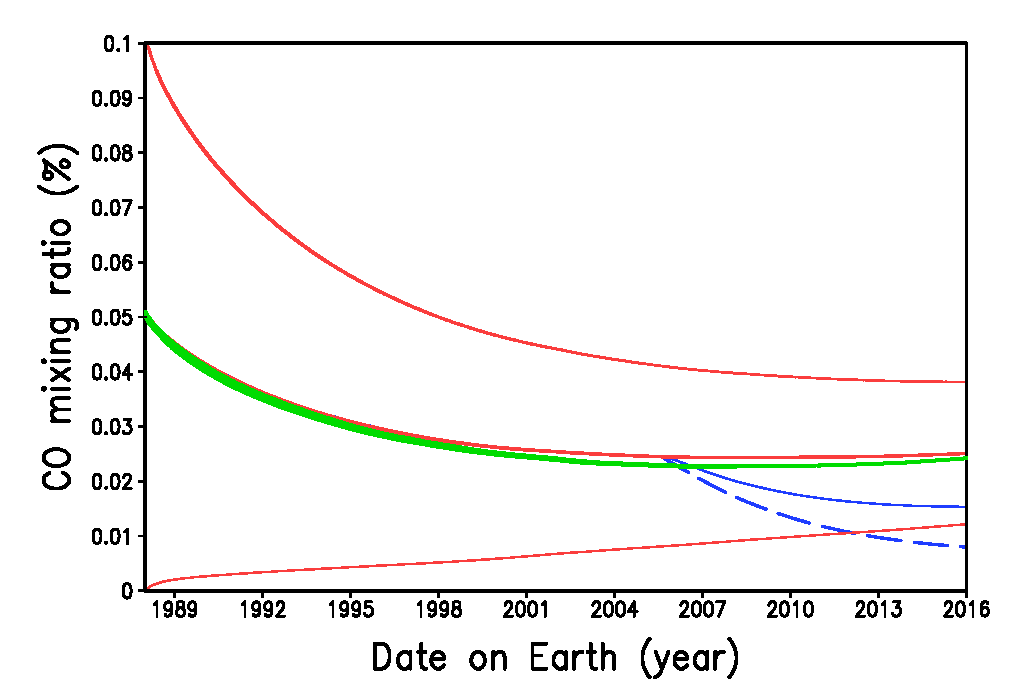
\includegraphics[width=12.cm,angle=-0,clip]{figures/evol_co.eps} \\
    \caption{
Evolution of the mean volume mixing ratio of gaseous carbon monoxide. The red curves
present the globally averaged values with different initialization. 
The green curve shows the apparent mixing ratio as seen from the Earth. The blue
curves shows the global mean mixing ratio in the alternative simulation 
with south pole N$_2$ condensation started in 2005 (see text). 
\label{fg:evol_co}
}
  \end{center}
\end{figure*}
%%%%%%%%%%%%%%%%%%%%%%%%%%%%%%%%%%%%%%%%%%%%%%%%%%%%%%%%%%%%%%%%%%%%%%

%%%%%%%%%%%%%%%%%%%%%%%%%%%%%%%%%%%%%%%%%%%%%%%%%%%%%%%%%%%%%%%%%%%%%%
% \begin{figure*}
%   \begin{center}
% \renewcommand{\arraystretch}{0.2}
% \renewcommand{\tabcolsep}{-0.0cm}
% \begin{tabular}[h]{ll}
% \hspace{-2cm}
% {\bf a) } & {\bf b) } \\
% \hspace{-2cm}
%     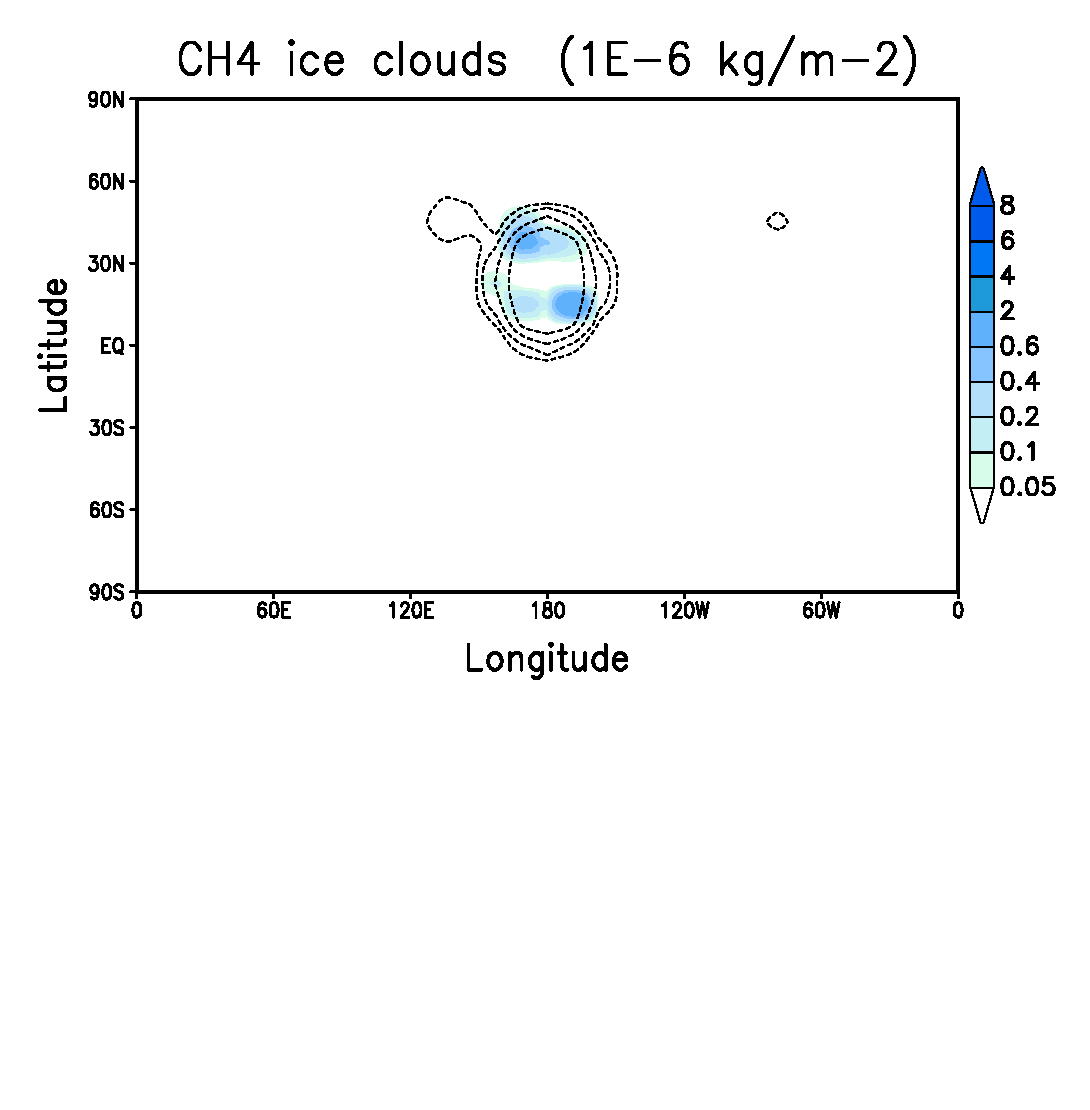
\includegraphics[height=6cm,angle=-0,clip]{figures/map_ch4clouds.eps} &
%     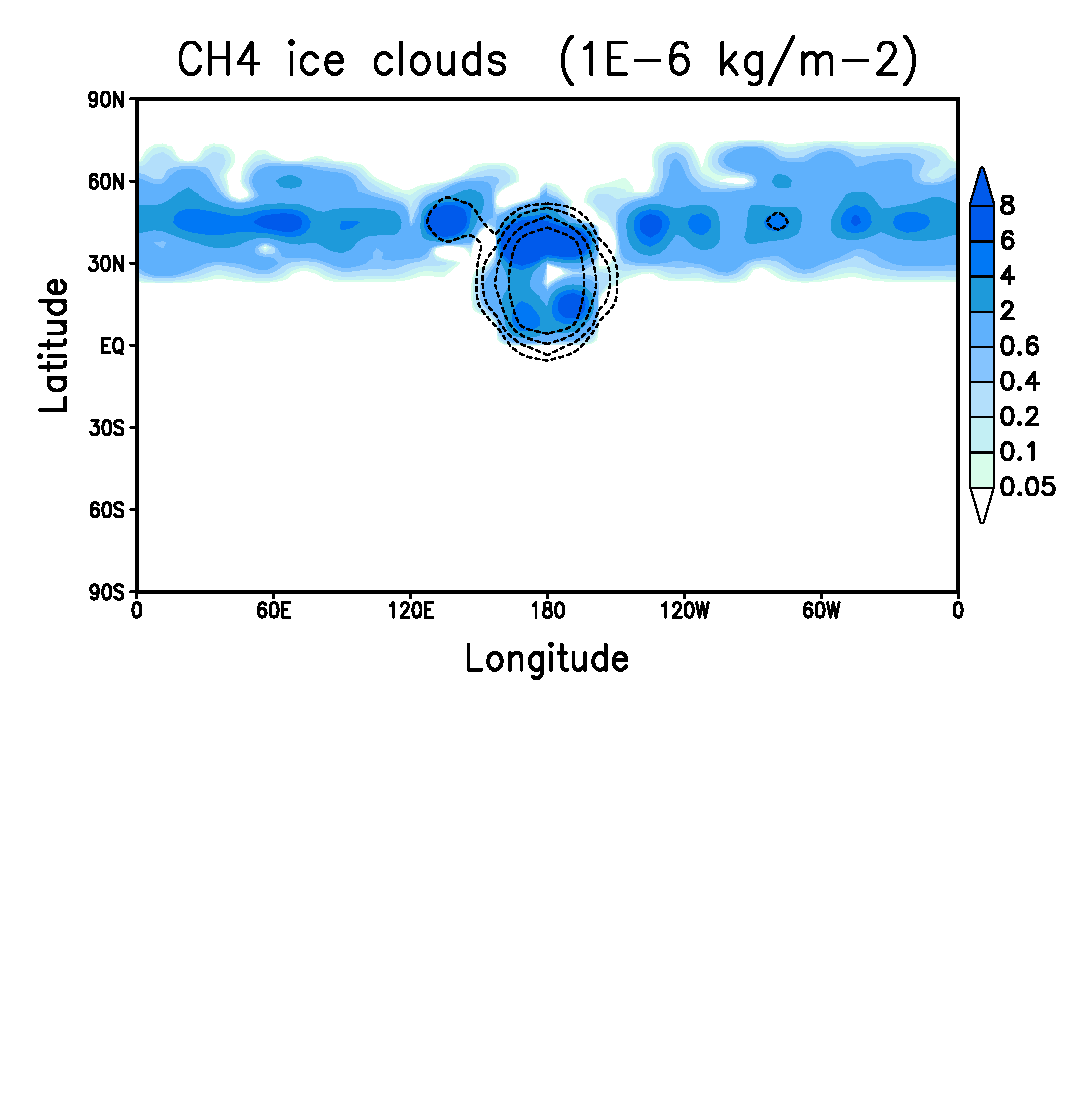
\includegraphics[height=6cm,angle=-0,clip]{figures/map_ch4clouds_pole.eps}
% \\
% \end{tabular}
%     \caption{
% Dayly-averaged map of methane ice clouds mass (1O$^-6$ kg per m$^2$) in July 2015 for the reference and
% alternative dimulations. 
% \label{fg:map_clouds} }
%   \end{center}
% \end{figure*}
%%%%%%%%%%%%%%%%%%%%%%%%%%%%%%%%%%%%%%%%%%%%%%%%%%%%%%%%%%%%%%%%%%%%%%


%%%%%%%%%%%%%%%%%%%%%%%%%%%%%%%%%%%%%%%%%%%%%%%%%%%%%%%%%%%%%%%%%%%%%%
% \begin{figure*}
%   \begin{center}
%    \includegraphics[width=12.cm,angle=-0,clip]{figures/section_clouds_t7.eps} \\
%    \includegraphics[width=12.cm,angle=-0,clip]{figures/section_clouds_t1.eps} \\
%    \includegraphics[width=12.cm,angle=-0,clip]{figures/section_clouds_t3.eps} \\
%    \includegraphics[width=12.cm,angle=-0,clip]{figures/section_clouds_t5.eps} \\ 
%     \caption{
% Crossection of Methane clouds at 45$^\circ$N as a function of longitude and altitude above the surface
% in the alternative simulation (with surface N$_2$ ice between 35$^\circ$N and 48$^\circ$N) around July 14 2015.
% The different pannels correspond to different times of days, as specified by the yellow line which provides a
% proxy of the local insolation. Note that CH$_2$ clouds are absent during the night. 
% \label{fg:section_clouds}
% }
%   \end{center}
% \end{figure*}
%%%%%%%%%%%%%%%%%%%%%%%%%%%%%%%%%%%%%%%%%%%%%%%%%%%%%%%%%%%%%%%%%%%%%%

\subsection{Conclusions}
%%%%%%%%%%%%%%%%%%%%%%%%

The goal of this paper was to describe, for the first time, our new Global Climate Model
of Pluto including the N$_2$, CH$_4$ and CO cycles. We presented two baseline
simulations which can shed light on New Horizons observations, for instance
to understand  the low
atmosphere temperature profiles measured by REX and the distribution of ices.
However, this is just the beginning. 
One of our key conclusions is that the Pluto climate system is extremely
sensitive to the assumed model parameters, such as the ice properties, the ground
thermal inertia, or the topography. Many more studies will have to be performed to
better simulate the reality and understand the processes at work. It
will also be very useful to perform longer simulations, with higher model resolution,
with a more realistic topography, etc...
We hope that this GCM will be applied to many specific studies
regarding clouds, hazes, frost deposits, seasonal evolution, and paleoclimates.  

%%%%%%%%%%%%%%%%%%%%%%%%%%%%%%%%%%%%%%%%%%%%%%%%%%%%%%%%%%%%%%%%%%%%
\section*{APPENDIX: Computing mass, momentum and heat vertical fluxes induced by N$_2$
condensation and sublimation in the GCM vertical coordinates}
%%%%%%%%%%%%%%%%%%%%%%%%%%%%%%%%%%%%%%%%%%%%%%%%%%%%%%%%%%%%%%%%%%%%

In the GCM, the changes in atmospheric mass due to the condensation and sublimation of nitrogen 
are taken into account by modifying the surface
pressure $p_0$ at each timestep by:
$\delta p_0 = -g \sum_{k=0}^{N}\delta m_k $,
with  $N$ the number of atmospheric model layers 
and $\delta m_k$ the mass condensed (or sublimed if $<0$) in layer $k$
or at the surface ($k=0$), as described in Section~\ref{sc:cond}.  
This ensures the conservation of the  total mass of N$_2$ (surface caps~+ atmosphere).

As described in Section~\ref{sc:dynamic}, 
the vertical coordinate of each model layer is defined by its
$\sigma_l = p_l/p_0$ coordinates. 
The changes in $p_0$  due to the N$_2$
condensation-sublimation induce ``artificial" movements of
the  $\sigma$ levels in the atmosphere.
This must be reflected in the temperature and wind fields.

Consider a
layer $l$ delimited by the levels $\sigma_{l-\dem}$
and  $\sigma_{l+\dem}$. At each timestep, its mass  $M_l =
\frac{p_0}{g}(\sigma_{l-\dem} -\sigma_{l+\dem})$ (in kg~m$^{-2}$)  
varies because of the global
variation of $p_0$. Such a variation $\delta M_l$ is associated with transfers
of mass between the layers (on which one must add the sink
corresponding to the local condensation $-\delta m_l$).  The local mass
balance may be written~:
\begin{equation}
\label{eq:dpdt1}
{\delta M_l} =
\frac{\delta p_0}{g}(\sigma_{l-\dem} -\sigma_{l+\dem})=
W_{l-\dem} - W_{l+\dem} - \delta m_l 
\end{equation}
where $W_{l-\dem}$ is the air mass (kg~m$^{-2}$) ``transfered''
through  the level $\sigma_{l-\dem}$ ($>0$ when up) during the timestep.
Equations~\ref{eq:dpdt1} can be rearanged to yield a  recursive formula on $W$~:
\begin{equation}
W_{l+\dem} = W_{l-\dem} - {\delta m_l} 
-\frac{\delta p_0}{g}(\sigma_{l-\dem} -\sigma_{l+\dem})
\end{equation}
with, in the first layer:
\begin{equation}
W_{\dem} = -\delta m_0
\end{equation}

The knowledge of $W$ can then be used
 to compute the exchange of
heat and momentum between the layers.
For $c_p T$ (enthalpy), the local heat balance can be written~:

\begin{equation}
\label{eq:transport1}
{\delta( M_l T_l)} = W_{l-\dem} \overline{T}_{l-\dem}
  - W_{l+\dem} \overline{T}_{l+\dem} - \delta m_l \ Tc_l
\end{equation}

with $\overline{T}_{l-\dem}$  the mean temperature of the gas transported
through the $\sigma_{l-\dem}$ interface.  
The calculation  of $\overline{T}_{l-\dem}$ is like in 
a classical transport problem. We use 
the ``Van-Leer~I'' finite volume transport scheme \citep{VanL:77,Hour:99}.
Separately, one can also write~:

\begin{equation}
\label{eq:transport2}
{\delta(M_l T_l)} =
 (M_l + \delta M_l) {\delta T_l} + T_l{\delta M_l }
\end{equation}

with  $\delta T_l$ the correction to be applied at every timestep
in each layer after the N$_2$ condensation or sublimation.
Eqs~\ref{eq:transport1} and ~\ref{eq:transport2} may be combined
to obtain $\delta T_l$

\begin{equation}
\label{eq:transport3}
\delta T_l = \frac{1}{M_l + \delta M_l}
[ W_{l-\dem} (\overline{T}_{l-\dem} - T_l)
- W_{l+\dem}(\overline{T}_{l+\dem} - T_l) - \delta m_l (Tc_l
-T_l) ]
\end{equation}

The first two terms, with $W_{l-\dem}$ and $W_{l+\dem}$, correspond to
the re-arrangement of the temperatures over the entire
column due to the pressure variations in $\sigma$ coordinates.
The last term $\delta m_l(Tc_l -T_l)$ is negligible
when N$_2$ condenses or partially sublimes since we then  have
 $Tc_l =  T_l$.  However, when  the N$_2$ totally sublimes
%(case of the equation~\ref{eq:subtot})
, it becomes
a cooling term  accounting for the mixing of the newly sublimed mass
$-\delta m_l$ with the rest of the layer at $T_l > Tc_l$.

On the ground, if $\delta m_0 > 0$  (condensation), we set $\overline{T}_{\dem} =
T_1$. 
As mentioned above, the near-surface cooling of the condensing 
N$_2$ gas from $T_1$ to $T_0$
is then taken into account in the surface energy balance.
If $\delta m_0 < 0$ (sublimation), we set  $\overline{T}_{\dem} =  T_0$.
The term $\delta m_0(T_0 - T_1)$ then accounts for the cooling of the lowest
level by the freshly-sublimed nitrogen.

Similarly, the momentum distribution must be re-arranged.  
For a wind component $v$, we shall simply write:

\begin{equation}
\delta v_l = \frac{1 }{M_l}
[ W_{l-\dem}(\overline{v}_{l-\dem} - v_l)
- W_{l+\dem}(\overline{v}_{l+\dem} - v_l)]
\end{equation}

with, on the ground,
$\overline{v}_{\dem} = v_1$ if $\delta m_0 > 0$
and  $\overline{v}_{\dem} = 0$ if $\delta m_0 < 0$
(the velocity of the N$_2$ gas that has just sublimed is zero).










%%%%%%%%%%%%%%%%%%%%%%%%%%%%%%%%%%%%%%%%%%%%%%%%%%%%%%%%%%%%%%%%%%%%
\section*{Acknowledgments}

The authors thank the NASA New Horizons team for their excellent work on a fantastic
mission and their interest in this research. We also thank CNES for its support. 
Finally, the authors are very grateful to two anonymous reviewers for their
exceptionally detailed comments which helped to improve the readibility of the article.

%%%%%%%%%%%%%%%%%%%%%%%%%%%%%%%%%%%%%%%%%%%%%%%%%%%%%%%%%%%%%%%%%%%%

